% CAVAT: bản 6 trang gửi REV-ECIT 2026. Bản chụp số liệu ngày 2026-10-16 (gen/ là bản sao, không tự cập nhật theo make paper-data).
% Biên dịch: tectonic main.tex
\documentclass[10pt,a4paper,twocolumn]{article}
% Phần mở đầu dùng chung của bài báo CAVAT (biên dịch bằng Tectonic / XeLaTeX).
\usepackage{fontspec}
% TeX Gyre: đủ dấu tiếng Việt, đi kèm bản phân phối TeX nên bài dựng giống nhau trên mọi máy
\setmainfont{texgyretermes}[Extension=.otf,UprightFont=*-regular,BoldFont=*-bold,ItalicFont=*-italic,BoldItalicFont=*-bolditalic]
\setsansfont{texgyreheros}[Extension=.otf,UprightFont=*-regular,BoldFont=*-bold,ItalicFont=*-italic,BoldItalicFont=*-bolditalic]
\setmonofont{texgyrecursor}[Extension=.otf,UprightFont=*-regular,BoldFont=*-bold,ItalicFont=*-italic,BoldItalicFont=*-bolditalic,Scale=0.92]
\usepackage{amsmath,amssymb}
\usepackage[a4paper,top=1.8cm,bottom=1.8cm,left=1.7cm,right=1.7cm,columnsep=0.65cm]{geometry}
\setlength{\headheight}{14pt}
\usepackage{booktabs,tabularx,array,multirow,makecell,longtable}
\usepackage{xcolor}
\usepackage{graphicx}
\usepackage{enumitem}
\usepackage{algorithm}
\usepackage{algpseudocode}
\usepackage{tikz}
\usetikzlibrary{arrows.meta,positioning,calc,fit,backgrounds,shapes.geometric,matrix,decorations.pathreplacing,patterns}
\usepackage{pgfplots}
\usepgfplotslibrary{groupplots,statistics}
\pgfplotsset{compat=1.18}
\usepackage[labelfont=bf,labelsep=period,font=small,justification=justified,singlelinecheck=false]{caption}
\usepackage{float}
\usepackage{placeins}
\usepackage{needspace}
\usepackage{microtype}
\usepackage{titlesec}
\usepackage{fancyhdr}
\definecolor{linkblue}{HTML}{000000}
\usepackage[colorlinks=true,linkcolor=linkblue,citecolor=linkblue,urlcolor=linkblue]{hyperref}

% --- màu
\definecolor{cavat}{HTML}{0072B2}
\definecolor{soft}{HTML}{F2F6FA}
\definecolor{llm}{HTML}{D55E00}
\definecolor{llmsoft}{HTML}{FBE5D6}
\definecolor{ink}{HTML}{1A1A1A}
\definecolor{mute}{HTML}{555555}
\definecolor{okgreen}{HTML}{009E73}
\definecolor{oksky}{HTML}{56B4E9}
\definecolor{okorange}{HTML}{E69F00}
\definecolor{rule}{HTML}{BFBFBF}
% vùng màu của khung đánh giá Toán (§25), trùng giao diện giáo viên
\definecolor{zoneE}{HTML}{EFF3FF}  % 0-39
\definecolor{zoneD}{HTML}{C6DBEF}  % 40-59
\definecolor{zoneC}{HTML}{6BAED6}  % 60-74
\definecolor{zoneB}{HTML}{3182BD}  % 75-89
\definecolor{zoneA}{HTML}{08519C}  % 90-100

% Màu hiện đại cho sơ đồ kiến trúc
\definecolor{cbluebg}{HTML}{EBF5FB}
\definecolor{cblueborder}{HTML}{2980B9}
\definecolor{cgreenbg}{HTML}{E8F8F5}
\definecolor{cgreenborder}{HTML}{27AE60}
\definecolor{cyellowbg}{HTML}{FEF9E7}
\definecolor{cyellowborder}{HTML}{D4AC0D}
\definecolor{credorangebg}{HTML}{FDEDEC}
\definecolor{credorangeborder}{HTML}{E74C3C}
\definecolor{cpurplebg}{HTML}{F5EEF8}
\definecolor{cpurpleborder}{HTML}{8E44AD}
\definecolor{cgraybg}{HTML}{F8F9F9}
\definecolor{cgrayborder}{HTML}{7F8C8D}

% --- tiếng Việt
\renewcommand{\abstractname}{Tóm tắt}
\renewcommand{\refname}{Tài liệu tham khảo}
\renewcommand{\figurename}{Hình}
\renewcommand{\tablename}{Bảng}
\renewcommand{\contentsname}{Mục lục}
\floatname{algorithm}{Thuật toán}
\renewcommand{\appendixname}{Phụ lục}
\algrenewcommand\algorithmicrequire{\textbf{Đầu vào:}}
\algrenewcommand\algorithmicensure{\textbf{Đầu ra:}}
\algrenewcommand\algorithmicif{\textbf{nếu}}
\algrenewcommand\algorithmicthen{\textbf{thì}}
\algrenewcommand\algorithmicelse{\textbf{ngược lại}}
\algrenewcommand\algorithmicfor{\textbf{với}}
\algrenewcommand\algorithmicforall{\textbf{với mọi}}
\algrenewcommand\algorithmicdo{\textbf{thực hiện}}
\algrenewcommand\algorithmicreturn{\textbf{trả về}}
\algrenewcommand\algorithmicwhile{\textbf{khi}}
\algrenewcommand\algorithmicend{\textbf{hết}}
\algrenewcommand\algorithmicuntil{\textbf{cho đến khi}}
\algrenewcommand\algorithmicrepeat{\textbf{lặp}}
\renewcommand{\algorithmiccomment}[1]{\hfill{\small\color{mute}\(\triangleright\) #1}}
\algnewcommand{\algorithmicinput}{\textbf{Đầu vào:}}

% --- bố cục
\setlength{\parindent}{1.2em}
\setlength{\parskip}{0pt}
\linespread{1.0}
\setlength{\emergencystretch}{3em}
\sloppy
\hbadness=10000
\titleformat{\section}{\normalsize\bfseries\color{ink}}{\thesection.}{0.6em}{\MakeUppercase}
\titleformat{\subsection}{\normalsize\bfseries\color{ink}}{\thesubsection}{0.5em}{}
\titleformat{\subsubsection}{\normalsize\itshape\color{ink}}{\thesubsubsection}{0.5em}{}
\titlespacing*{\section}{0pt}{1.4ex plus 0.2ex minus 0.1ex}{0.5ex plus 0.1ex}
\titlespacing*{\subsection}{0pt}{1.1ex plus 0.2ex minus 0.1ex}{0.4ex plus 0.1ex}
\titlespacing*{\subsubsection}{0pt}{0.9ex plus 0.2ex minus 0.1ex}{0.3ex plus 0.1ex}
\setlist{nosep,leftmargin=1.6em,itemsep=1.5pt}
\captionsetup[table]{skip=4pt}
\captionsetup[figure]{skip=4pt}
\renewcommand{\arraystretch}{1.08}
\newcolumntype{Y}{>{\raggedright\arraybackslash}X}
\newcolumntype{C}{>{\centering\arraybackslash}X}
\newcolumntype{R}[1]{>{\raggedleft\arraybackslash}p{#1}}
\newcommand{\vn}[1]{\textit{#1}}
\newcommand{\code}[1]{\texttt{\small #1}}
\newcommand{\rid}[1]{\textsf{\small #1}}   % mã luật: R-..., N-...
\newcommand{\DI}[1]{\textsf{DI-#1}}
\newcommand{\tick}{\textcolor{cavat}{\(\bullet\)}}
\newcommand{\best}[1]{\textbf{#1}}

% --- số thập phân dùng dấu phẩy trong biểu đồ
\pgfplotsset{
  cavat/.style={
    /pgf/number format/use comma,
    /pgf/number format/precision=2,
    /pgf/number format/fixed,
    /pgf/number format/fixed zerofill=false,
    tick label style={font=\scriptsize},
    label style={font=\small},
    legend style={font=\scriptsize,draw=none,fill=none},
    title style={font=\small\bfseries},
    axis line style={color=ink},
    grid style={color=rule,line width=0.3pt},
    every axis plot/.append style={line width=0.9pt},
  }
}

% --- thả nổi: giữ bảng và hình trong mục của nó
\renewcommand{\topfraction}{0.95}
\renewcommand{\bottomfraction}{0.85}
\renewcommand{\textfraction}{0.05}
\renewcommand{\floatpagefraction}{0.75}
\setcounter{topnumber}{4}
\setcounter{bottomnumber}{3}
\setcounter{totalnumber}{6}

\let\OldSection\section
\renewcommand{\section}{\Needspace*{4\baselineskip}\OldSection}
\renewcommand{\sectionmark}[1]{\markright{#1}}
\let\OldSubsection\subsection
\renewcommand{\subsection}{\Needspace*{3\baselineskip}\OldSubsection}

% --- bố cục hai cột kiểu bài hội nghị
\setlength{\columnseprule}{0pt}
\renewcommand{\dbltopfraction}{0.95}
\renewcommand{\dblfloatpagefraction}{0.75}
\setcounter{dbltopnumber}{4}
\setlength{\dbltextfloatsep}{8pt plus 2pt minus 2pt}
\setlength{\textfloatsep}{8pt plus 2pt minus 2pt}
\setlength{\abovecaptionskip}{3pt}
\setlength{\belowcaptionskip}{0pt}
\captionsetup{font={small}}
% khối tiêu đề và tóm tắt trải hai cột: hộp tóm tắt nền nhạt
\newsavebox{\absbox}
\renewenvironment{abstract}{%
  \begin{lrbox}{\absbox}\begin{minipage}{0.94\textwidth}\vspace{3pt}\small\noindent\textbf{Tóm tắt.}\ }{%
  \vspace{2pt}\end{minipage}\end{lrbox}%
  \begin{center}\usebox{\absbox}\end{center}\vspace{-3pt}}

% URL dài trong tài liệu tham khảo được phép ngắt ở bất kỳ chữ nào
\makeatletter
\g@addto@macro\UrlBreaks{\do\a\do\e\do\i\do\o\do\t\do\n\do\s\do\r\do\l\do\c\do\-}
\makeatother

% Sinh tự động từ docs/paper/data/*.json bởi services/api/scripts/paper_figures.py. Không sửa tay.
\providecommand{\NDocs}{18}
\providecommand{\NDocsDec}{9}
\providecommand{\NDocsGeo}{9}
\providecommand{\NPages}{77}
\providecommand{\NPagesDec}{38}
\providecommand{\NPagesGeo}{39}
\providecommand{\NSyll}{24\,920}
\providecommand{\NPagesText}{46}
\providecommand{\NPagesOcr}{31}
\providecommand{\NOcrImages}{12}
\providecommand{\NOcrFigure}{19}
\providecommand{\NNumbersAdded}{27}
\providecommand{\NConfirmedPages}{6}
\providecommand{\NDisputedNumbers}{5}
\providecommand{\NReviewPages}{2}
\providecommand{\NItems}{389}
\providecommand{\NItemsDec}{234}
\providecommand{\NItemsGeo}{155}
\providecommand{\NVerified}{349}
\providecommand{\NConflict}{2}
\providecommand{\NDisputedItems}{1}
\providecommand{\NReviewItems}{4}
\providecommand{\NUnchecked}{33}
\providecommand{\NAssess}{79}
\providecommand{\NFigureItems}{19}
\providecommand{\NNodes}{19}
\providecommand{\NNodesDec}{11}
\providecommand{\NNodesGeo}{8}
\providecommand{\NEdges}{28}
\providecommand{\NEdgesPrereq}{9}
\providecommand{\NEdgesApp}{19}
\providecommand{\NPlanItems}{381}
\providecommand{\NPlanHints}{698}
\providecommand{\NMisconceptions}{54}
\providecommand{\NCritical}{16}
\providecommand{\NDrafts}{1\,379}
\providecommand{\NDraftsOk}{969}
\providecommand{\NDraftsQwen}{771}
\providecommand{\NDraftsFallback}{608}
\providecommand{\NDecisions}{1\,326}
\providecommand{\NApprove}{1\,112}
\providecommand{\NEdit}{129}
\providecommand{\NReject}{85}
\providecommand{\NChunks}{221}
\providecommand{\NChunksDec}{115}
\providecommand{\NChunksGeo}{106}
\providecommand{\NPassages}{83}
\providecommand{\NPassagesTied}{29}
\providecommand{\NPassagesSpread}{54}
\providecommand{\NChunksSample}{47}
\providecommand{\NVecDim}{768}
\providecommand{\NQuestions}{180}
\providecommand{\NQuestionsInScope}{124}
\providecommand{\NEventsDec}{1\,654}
\providecommand{\NEventsGeo}{1\,101}
\providecommand{\NEvents}{2\,755}
\providecommand{\NTutorMsg}{468}
\providecommand{\NLeakChecked}{308}
\providecommand{\NLeaks}{0}
\providecommand{\NStudentMsg}{403}
\providecommand{\NItemsResolved}{142}
\providecommand{\NDIs}{58}
\providecommand{\TargetMean}{85\%}

\renewcommand{\thesection}{\Roman{section}}
\renewcommand{\thesubsection}{\thesection.\Alph{subsection}}
\title{CAVAT}\author{Dương Minh Vương, Nguyễn Quốc Bảo, Đỗ Ngọc Minh}\date{}

\pagestyle{fancy}
\fancyhf{}
\renewcommand{\headrulewidth}{0.4pt}
\renewcommand{\headrule}{\hbox to\headwidth{\color{rule}\leaders\hrule height \headrulewidth\hfill}}
\fancyhead[L]{\footnotesize\itshape Tách quyết định sư phạm khỏi mô hình ngôn ngữ}
\fancyhead[R]{\footnotesize\itshape\nouppercase{\rightmark}}
\fancyfoot[C]{\small\thepage}
\fancypagestyle{first}{\fancyhf{}\renewcommand{\headrulewidth}{0pt}\fancyfoot[C]{\small\thepage}}

\makeatletter
\renewcommand{\dbltopfraction}{0.95}
\setlength\@dblfptop{0pt}
\setlength\@dblfpsep{6pt}
\setlength\@dblfpbot{0pt plus 1fil}
\makeatother

\begin{document}
\twocolumn[{%
% Header theo mẫu REV-ECIT: banner REV-ECIT 2026 (rev-ecit-2026-header.jpg, dựng từ mẫu poster 2024: lần thứ XXIX,
% logo Bộ KH&CN, REV, Cục Tần số Vô tuyến điện) phủ hết bề ngang trang; tên bài, tác giả, đơn vị nằm trên phần nền xanh.
\begin{tikzpicture}[remember picture,overlay]
  \node[anchor=north,inner sep=0pt] at (current page.north)
    {
\includegraphics[width=\paperwidth]{rev-ecit-2026-header.jpg}};
  \node[anchor=north,inner sep=0pt,text width=0.9\paperwidth,align=center,text=white]
    at ([yshift=-30.5mm]current page.north) {%
    {\fontsize{14}{16.5}\selectfont\bfseries
     TÁCH QUYẾT ĐỊNH SƯ PHẠM KHỎI MÔ HÌNH NGÔN NGỮ:\\
     GIA SƯ TOÁN SOCRATIC VỚI TRUY XUẤT LAI THEO ĐỒ THỊ TRI THỨC\par}
    \vspace{5pt}
    {\fontsize{10}{12.5}\selectfont
     \textbf{\textit{Tác giả:}} Dương Minh Vương, Nguyễn Quốc Bảo, Đỗ Ngọc Minh\par
     \textbf{\textit{Đơn vị:}} Trường Đại học Công nghệ, Đại học Quốc gia Hà Nội\par}
  };
\end{tikzpicture}%
% chừa chỗ cho banner: cao 210 mm x 720/2383 = 63,45 mm tính từ mép trên trang, trừ lề trên 1,8 cm
\vspace*{\dimexpr 63.45mm - 1.8cm - 1.5mm\relax}
\begin{center}
{\fontsize{9.5}{11.5}\selectfont\itshape
Decoupling Pedagogical Decisions from the Language Model: a Socratic Grade-5 Mathematics Tutor\\
with Graph-Constrained Hybrid Retrieval and a Replayable Learner Model\par}
\end{center}
\vspace{-8pt}
\begin{abstract}
\noindent
Việc ứng dụng mô hình ngôn ngữ lớn (LLM) trong các hệ thống gia sư thông minh đặt ra thách thức lớn về khả năng kiểm soát hành vi sư phạm và tính phù hợp của nội dung hỗ trợ. Bài báo đề xuất CAVAT, một kiến trúc gia sư Toán lớp 5 theo phương pháp Socratic, trong đó các quyết định sư phạm, đánh giá câu trả lời và cập nhật trạng thái người học được thực hiện bởi các thành phần tất định, trong khi LLM chỉ đảm nhiệm vai trò diễn đạt phản hồi dưới sự giám sát của bộ kiểm chứng an toàn. Hệ thống kết hợp truy xuất từ khóa và ngữ nghĩa với đồ thị tri thức nhằm giới hạn nội dung theo đúng tiến trình học tập, đồng thời sử dụng cơ chế định tuyến chủ đề để duy trì độ chính xác truy xuất. Thực nghiệm trên hai chương Toán lớp 5 cho thấy phương pháp đạt Hit@3 = 0,90, tương đương với Flat RAG không ràng buộc, nhưng loại bỏ hoàn toàn việc truy xuất trước kiến thức bài sau vào ba kết quả đầu (0/30 so với 12/30). Trong các tình huống hội thoại mô phỏng, CAVAT không ghi nhận bất kỳ lượt tiết lộ đáp án nào (0/24), so với 1/25 ở cấu hình chỉ sử dụng lời nhắc Socratic và 15/25 ở chatbot thương mại thông thường. Kết quả khẳng định tính khả thi của kiến trúc tách quyết định sư phạm khỏi quá trình sinh ngôn ngữ, tạo cơ sở phát triển gia sư AI có hành vi kiểm soát được và năng lực đánh giá tái lập hoàn toàn.

\vspace{2pt}
\noindent\textbf{Từ khóa:} Gia sư thông minh; mô hình ngôn ngữ lớn; phương pháp Socratic; truy xuất tăng cường (RAG); đồ thị tri thức; mô hình người học.
\end{abstract}
\vspace{2pt}
}]
\thispagestyle{first}

\section{Giới thiệu chung}\label{sec:intro}

% ==================== HÌNH 1: KIẾN TRÚC CAVAT (XUẤT HIỆN Ở ĐẦU TRANG 2) ====================
% Vẽ ngoài LaTeX: nguồn fig-architecture.svg (sửa được bằng Inkscape, draw.io, Figma), xuất ra fig-architecture.pdf.
\begin{figure*}[t]
\centering
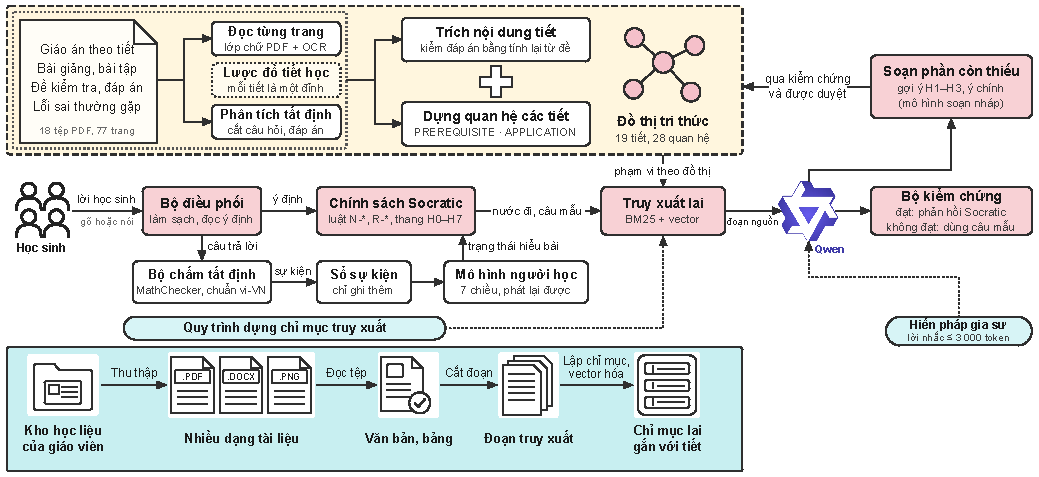
\includegraphics[width=\textwidth]{fig-architecture.pdf}
\caption{Kiến trúc tổng thể của CAVAT. Vùng trên: dựng đồ thị tri thức từ tài liệu của giáo viên (đọc từng trang, phân tích tất định, trích nội dung tiết kèm kiểm đáp án, dựng quan hệ giữa các tiết); phần do mô hình ngôn ngữ soạn nháp (gợi ý, ý chính) chỉ vào phương án khi qua kiểm chứng và được duyệt. Vùng giữa: một lượt dạy, trong đó bộ điều phối, chính sách Socratic, bộ chấm, sổ sự kiện và mô hình người học đều tất định; mô hình ngôn ngữ (Qwen) chỉ diễn đạt nước đi và câu mẫu, và lời của nó chỉ đến học sinh khi qua bộ kiểm chứng (bất biến B1--B6). Vùng dưới: dựng chỉ mục truy xuất lai từ tài liệu và phương án đã duyệt.}\label{fig:arch}
\end{figure*}

Việc dạy kèm từ lâu đã được chứng minh là một trong những can thiệp sư phạm hiệu quả nhất trong giáo dục~\cite{bloom1984,vanlehn2011}. Sự bùng nổ của các mô hình ngôn ngữ lớn (LLM) mở ra tiềm năng phổ cập trợ lý học tập cá nhân hóa đến đông đảo người học. Tuy nhiên, các mô hình tạo sinh tiềm ẩn rủi ro sư phạm nghiêm trọng: mô hình thường có xu hướng giải bài hộ hoặc đưa ra đáp án trực tiếp cho học sinh~\cite{macina2023,tack2022}. Nghiên cứu thực nghiệm gần đây cho thấy người học dùng trợ lý AI thiếu cơ chế kiểm soát có thể cải thiện kết quả tức thời khi làm bài nhưng suy giảm rõ rệt thành tích trong các kỳ đánh giá độc lập~\cite{bastani2025}. Dù hệ thống gia sư tuân thủ nghiêm ngặt nguyên tắc sư phạm mang lại hiệu quả vượt trội~\cite{kestin2025}, thách thức cốt lõi là bảo đảm các nguyên tắc này luôn được thực thi tin cậy.

Hiện nay, các giải pháp thương mại thường bổ sung ``chế độ học tập'' (study mode)~\cite{studymode,guidedlearning,khanmigo}. Tuy nhiên, ràng buộc sư phạm trong các hệ thống này chỉ tồn tại dưới dạng hướng dẫn ngữ cảnh (prompting), trong đó LLM vẫn trực tiếp ra quyết định hành vi. Khi người học khăng khăng bảo vệ đáp án sai, yêu cầu cung cấp ngay lời giải hoặc thực hiện tấn công bỏ qua chỉ dẫn (jailbreak/prompt injection)~\cite{perez2022}, hệ thống hoàn toàn thiếu vắng cơ chế kỹ thuật để bảo đảm hành vi sư phạm chuẩn mực.

Nghiên cứu này tiếp cận việc ra quyết định sư phạm (chọn câu hỏi, xác định bậc gợi ý, kiểm soát điểm dừng) như một bài toán điều khiển có trạng thái, được hình thức hóa bằng tập luật tường minh và kiểm chứng tất định; LLM chỉ đóng vai trò chuyển hóa quyết định thành ngôn ngữ tự nhiên. Giả thuyết nghiên cứu là: khi các khâu quyết định sư phạm, đánh giá đúng--sai và cập nhật trạng thái người học được giao hoàn toàn cho các thành phần tất định, tỉ lệ tiết lộ đáp án sẽ triệt tiêu về 0\% trong khi chất lượng diễn đạt vẫn đạt chuẩn sư phạm và kiểm chứng được bằng luật.

Kiến trúc phân tách này đặt ra thách thức: hệ thống phải bám sát học liệu chuẩn của giáo viên mà không được tiết lộ trước kiến thức bài học phía sau. Phương pháp RAG tiêu chuẩn (Flat RAG) không có khái niệm ``bài chưa học'' theo tiến trình; do đó, nghiên cứu mô hình hóa bài học thành đồ thị tri thức để ràng buộc không gian tìm kiếm. Để bù đắp độ bao phủ khi học sinh hỏi lại kiến thức cũ, cơ chế định tuyến chủ đề (topic routing) đề xuất đã khôi phục toàn diện độ chính xác của hệ thống. Các đóng góp chính của bài báo gồm:
\begin{enumerate}
  \item Đề xuất kiến trúc CAVAT phân tách quyết định sư phạm khỏi LLM: chính sách tất định điều phối nước đi, bộ chấm tất định đánh giá câu trả lời, mô hình người học tái lập từ sổ sự kiện, và LLM diễn đạt dưới sự giám sát của bộ kiểm chứng an toàn.
  \item Thiết kế cơ chế truy xuất lai ràng buộc theo đồ thị tri thức kết hợp định tuyến chủ đề từ nguồn tài liệu thực tế của giáo viên tiểu học.
  \item Xây dựng giao thức đánh giá đa chiều trên các tập dữ liệu đóng băng, đối chứng toàn diện với Flat RAG, chatbot thương mại và cấu hình LLM chỉ dựa trên lời nhắc (prompt-only).
  \item Kiểm chứng thực nghiệm độ bám sát khung đánh giá năng lực môn Toán thông qua đối chiếu tiêu chí, kiểm thử tương đương công thức đóng và phân tích đường đáp ứng.
\end{enumerate}

\section{Công trình liên quan}\label{sec:related}

\textbf{Gia sư thông minh và gia sư dựa trên LLM.} Các hệ thống gia sư thông minh (ITS) truyền thống tập trung điều tiết mức hỗ trợ sư phạm tối ưu thông qua kỹ thuật giàn giáo giảm dần~\cite{wood1976}, nghịch lý hỗ trợ~\cite{koedinger2007,aleven2016} và hiệu ứng đảo ngược chuyên môn~\cite{kalyuga2003}; tiêu biểu như AutoTutor~\cite{graesser2005} tự động hóa hội thoại bằng luật tất định nhưng khả năng diễn đạt còn hạn chế. Gần đây, LearnLM-Tutor~\cite{jurenka2024} và SocraticLM~\cite{liu2024socratic} khai thác LLM nhằm tăng độ linh hoạt hội thoại, song việc để mô hình tự quyết định hành vi vẫn tiềm ẩn rủi ro tiết lộ lời giải hoặc phản hồi sai lệch~\cite{macina2023,tack2022}. Hệ thống CAVAT khắc phục hạn chế này bằng cách kế thừa cơ chế điều khiển tất định của ITS và chỉ xem LLM như công cụ sinh ngôn ngữ tự nhiên.

\textbf{Truy xuất tăng cường (RAG).} Các phương pháp RAG hiện đại~\cite{lewis2020} thường kết hợp thuật toán BM25~\cite{robertson2009}, truy xuất ngữ nghĩa dày đặc~\cite{karpukhin2020} và xếp hạng tương hỗ RRF~\cite{cormack2009}; trong khi Graph RAG~\cite{edge2024} khai thác đồ thị để tổng hợp thông tin diện rộng. Dù vậy, các hệ thống Flat RAG và Graph RAG hiện hữu đều thiếu khái niệm tiến trình học tập. CAVAT sử dụng đồ thị tri thức như không gian ràng buộc sư phạm nghiêm ngặt, ngăn chặn triệt để việc truy xuất kiến thức thuộc bài học phía sau.

\textbf{Mô hình người học và phương pháp đánh giá.} Các mô hình vết tri thức Bayesian~\cite{corbett1995,pelanek2017} hay mạng nơ-ron sâu~\cite{piech2015} đạt hiệu quả dự báo tốt nhưng thiếu tính giải thích sư phạm. CAVAT mô hình hóa năng lực bằng phân phối Beta đa chiều, cho phép ánh xạ tường minh với khung chuẩn năng lực. Trong khâu đánh giá, mô hình LLM-as-a-judge~\cite{zheng2023} chỉ chấm độ tự nhiên phát ngôn; các chỉ số an toàn sư phạm đều được kiểm chứng tất định kết hợp các kiểm định thống kê chuẩn xác~\cite{wilson1927,efron1993,mcnemar1947}.

\section{Phương pháp đề xuất}\label{sec:method}

\subsection{Kiến trúc tổng thể và các bất biến sư phạm}
Hình~\ref{fig:arch} mô tả kiến trúc của CAVAT. Trong mỗi lượt đối thoại, bộ điều phối chuẩn hóa dữ liệu và nhận diện ý định của học sinh. Dựa trên vị trí bài học trên đồ thị tri thức, chính sách sư phạm xác định nước đi tương tác cùng mức gợi ý phù hợp. Bộ chấm tất định kiểm tra tính đúng--sai của câu trả lời. LLM tiếp nhận nước đi, câu mẫu chuẩn và đoạn học liệu nguồn để diễn đạt phản hồi tự nhiên. Bộ kiểm chứng an toàn rà soát phát ngôn dự thảo; nếu phát hiện vi phạm (tiết lộ đáp án, đặt nhiều câu hỏi, quá dài hoặc thiếu nguồn dẫn), hệ thống lập tức thay thế bằng câu mẫu an toàn của giáo viên.

Kiến trúc bảo đảm sáu bất biến sư phạm cốt lõi:
(B1) đáp án câu hỏi kiểm tra không bao giờ được đưa vào ngữ cảnh LLM;
(B2) chính sách tất định quyết định nước đi, LLM chỉ đảm nhiệm diễn đạt;
(B3) kết luận đúng--sai do bộ chấm tất định thực hiện;
(B4) điểm số năng lực là phép chiếu toán học tái lập hoàn toàn từ sổ sự kiện;
(B5) hệ thống không giảng dạy trước nội dung bài học phía sau;
(B6) mọi khẳng định của gia sư đều có căn cứ trực tiếp từ học liệu nguồn hoặc phát ngôn của học sinh. Mọi ràng buộc đều do máy chủ kiểm soát tập trung.

% ==================== COMPOSITE FLOAT 1: TOÀN BỘ KẾT QUẢ TRUY XUẤT (KHAI BÁO Ở ĐÂY ĐỂ VÀO ĐẦU TRANG 3) ====================
\begin{figure*}[t]
\centering
\begin{minipage}[t]{0.45\textwidth}\vspace{0pt}
\captionof{table}{Mức đạt so với bảy định hướng thiết kế của truy xuất. Mức đạt $=\min(1,\text{đo được}/\text{mục tiêu})$.}\label{tab:targets}
\footnotesize
\begin{tabularx}{\linewidth}{@{}lYlrr@{}}
\toprule
Mã & Định hướng thiết kế & Mục tiêu & Đo được & Mức đạt \\
\midrule
R1 & Truy xuất đúng đoạn tri thức cho câu hỏi trong bài (Hit@3) & $\geq 0{,}90$ & 0,87 & 96\% \\
R2 & Câu lạc đề, Toán ngoài chương không bị trả lời & $\geq 95\%$ & 100\% & 100\% \\
R3 & Câu hỏi trong chương được xác nhận có căn cứ & $\geq 95\%$ & 95\% & 100\% \\
R4 & Ngăn chặn hoàn toàn việc dạy trước nội dung bài sau & $100\%$ & 100\% & 100\% \\
R5 & Phản hồi bám sát nguồn học liệu (giám khảo, thang 5) & $\geq 95\%$ & 100\% & 100\% \\
R6 & Lượt bịa hoặc lộ đáp án & $\leq 2\%$ & 0\% & 100\% \\
R7 & Truy xuất lai + xếp hạng lại tốt nhất (MRR) & có/không & không & 0\% \\
\midrule
\multicolumn{4}{@{}l}{Mức đạt trung bình của bảy định hướng thiết kế} & \textbf{85\%} \\
\bottomrule
\end{tabularx}

\end{minipage}\hfill
\begin{minipage}[t]{0.52\textwidth}\vspace{0pt}
\captionof{table}{So sánh CAVAT (ràng buộc đồ thị) với Flat RAG. ``Đoạn bài sau'': số câu có đoạn của tiết chưa học trong top-3.}\label{tab:flat}
\footnotesize
\setlength{\tabcolsep}{3pt}
\begin{tabular}{@{}llrrrrr@{}}
\toprule
Tập & Hệ truy xuất & Hit@3 & MRR & \makecell{Đoạn bài sau\\trong top-3} & \makecell{Câu bài sau\\bị trả lời} & \makecell{Câu ngoài\\chương bị trả lời} \\
\midrule
Bộ chỉnh & CAVAT (ràng buộc đồ thị) & 1,00 & 0,944 & 0/30 & 0/4 & 0/8 \\
 & Flat RAG & 1,00 & 0,907 & 10/30 & 4/4 & 1/8 \\
 & Flat RAG + xếp hạng lại & 1,00 & 0,880 & 12/30 & 4/4 & 1/8 \\
\midrule
Giữ riêng v1 & CAVAT (ràng buộc đồ thị) & 1,00 & 0,952 & 0/23 & 0/3 & 0/6 \\
 & Flat RAG & 0,86 & 0,806 & 9/23 & 3/3 & 1/6 \\
 & Flat RAG + xếp hạng lại & 0,86 & 0,787 & 9/23 & 3/3 & 1/6 \\
\midrule
Giữ riêng v2 & CAVAT (ràng buộc đồ thị) & 0,90 & 0,887 & 0/30 & 0/4 & 0/6 \\
 & Flat RAG & 0,90 & 0,873 & 12/30 & 4/4 & 1/6 \\
 & Flat RAG + xếp hạng lại & 0,90 & 0,848 & 11/30 & 4/4 & 1/6 \\
\bottomrule
\end{tabular}

\end{minipage}
\vspace{4pt}
\begin{tikzpicture}
\begin{groupplot}[group style={group size=3 by 1,horizontal sep=1.0cm,y descriptions at=edge left},cavat,width=5.6cm,height=4.8cm,ymin=0.3,ymax=1.03,xmin=1,xmax=10,xtick={1,3,5,7,10},ymajorgrids,xlabel={$k$},]
\nextgroupplot[title={(a) bộ chỉnh},ylabel={Hit@$k$}]
\addplot[color=ink!60,dashed,line width=0.9pt,mark=square*,mark size=1.4pt] coordinates {(1,0.722) (2,0.833) (3,0.833) (4,0.833) (5,0.944) (6,0.944) (7,0.944) (8,0.944) (9,0.944) (10,0.944)};
\addplot[color=cavat,solid,line width=0.9pt,mark=*,mark size=1.4pt] coordinates {(1,0.889) (2,1.000) (3,1.000) (4,1.000) (5,1.000) (6,1.000) (7,1.000) (8,1.000) (9,1.000) (10,1.000)};
\addplot[color=llm,dotted,line width=0.9pt,mark=triangle*,mark size=1.4pt] coordinates {(1,0.833) (2,0.944) (3,1.000) (4,1.000) (5,1.000) (6,1.000) (7,1.000) (8,1.000) (9,1.000) (10,1.000)};
\nextgroupplot[title={(b) giữ riêng v1}]
\addplot[color=ink!60,dashed,line width=0.9pt,mark=square*,mark size=1.4pt] coordinates {(1,0.643) (2,0.643) (3,0.643) (4,0.643) (5,0.714) (6,0.714) (7,0.714) (8,0.786) (9,0.857) (10,0.857)};
\addplot[color=cavat,solid,line width=0.9pt,mark=*,mark size=1.4pt] coordinates {(1,0.929) (2,0.929) (3,1.000) (4,1.000) (5,1.000) (6,1.000) (7,1.000) (8,1.000) (9,1.000) (10,1.000)};
\addplot[color=llm,dotted,line width=0.9pt,mark=triangle*,mark size=1.4pt] coordinates {(1,0.714) (2,0.857) (3,0.857) (4,0.857) (5,0.857) (6,0.929) (7,0.929) (8,0.929) (9,1.000) (10,1.000)};
\nextgroupplot[title={(c) giữ riêng v2}]
\addplot[color=ink!60,dashed,line width=0.9pt,mark=square*,mark size=1.4pt] coordinates {(1,0.450) (2,0.450) (3,0.450) (4,0.450) (5,0.450) (6,0.600) (7,0.650) (8,0.700) (9,0.750) (10,0.800)};
\addplot[color=cavat,solid,line width=0.9pt,mark=*,mark size=1.4pt] coordinates {(1,0.850) (2,0.900) (3,0.900) (4,0.900) (5,0.900) (6,0.950) (7,0.950) (8,0.950) (9,0.950) (10,0.950)};
\addplot[color=llm,dotted,line width=0.9pt,mark=triangle*,mark size=1.4pt] coordinates {(1,0.800) (2,0.900) (3,0.900) (4,0.950) (5,1.000) (6,1.000) (7,1.000) (8,1.000) (9,1.000) (10,1.000)};
\end{groupplot}
\end{tikzpicture}
\\[3pt]
\begin{tikzpicture}[x=1cm,y=1cm]
\draw[color=ink!60,dashed,line width=0.9pt] (-0.15,0) -- (0.45,0);
\node[circle,fill=none,inner sep=0pt] at (0.15,0) {};
\node[anchor=west,font=\scriptsize,inner sep=1pt] at (0.62,0) {không định tuyến};
\draw[color=cavat,line width=0.9pt] (3.08,0) -- (3.68,0);
\node[circle,fill=none,inner sep=0pt] at (3.38,0) {};
\node[anchor=west,font=\scriptsize,inner sep=1pt] at (3.85,0) {có định tuyến (sản phẩm)};
\draw[color=llm,dotted,line width=0.9pt] (7.39,0) -- (7.99,0);
\node[circle,fill=none,inner sep=0pt] at (7.69,0) {};
\node[anchor=west,font=\scriptsize,inner sep=1pt] at (8.16,0) {Flat RAG (không đồ thị)};
\end{tikzpicture}

\caption{Hit@$k$ của cấu hình sản phẩm khi có và không có định tuyến, so sánh với Flat RAG trên ba tập dữ liệu kiểm thử.}\label{fig:hitk}
\end{figure*}

\subsection{Chính sách Socratic và thang gợi ý}
Chính sách sư phạm hoạt động theo tập luật tường minh có quản lý phiên bản, áp dụng nguyên tắc hỗ trợ tối thiểu cần thiết qua thang gợi ý tám bậc $H_0$--$H_7$ (từ câu hỏi định hướng, nhắc khái niệm đến giải thích từng bước) với trọng số suy giảm $\iota_h \in \{1{,}0;\,0{,}85;\,0{,}70;\,0{,}60;\,0{,}50;\,0{,}35;\,0{,}20;\,0\}$. Học sinh luôn bắt đầu ở mức hỗ trợ thấp nhất; bậc gợi ý chỉ tăng khi gặp khó khăn và được rút lại ngay khi hoàn thành một bước độc lập. Chỉ mức $H_7$ mới cung cấp lời giải đầy đủ trong phiên luyện tập; ở phiên kiểm tra, mức hỗ trợ tối đa bị chặn ở $H_1$. Các phản hồi ngoài lề được nhận diện riêng và không tính là lỗi sai. Quy trình ra quyết định là hàm tất định theo trạng thái phiên học, bảo đảm tính tái lập hoàn toàn.

\subsection{Truy xuất lai ràng buộc theo đồ thị tri thức}
Đồ thị bài học $G=(V,E)$ xác định cấu trúc chương trình với các đỉnh tiết học và cạnh quan hệ tiên quyết (\textsc{prerequisite}), vận dụng (\textsc{application}). Mỗi đoạn tri thức $c$ gắn liền với một tiết học $\nu(c)$. Khi người học đặt câu hỏi tại tiết $v$, không gian tìm kiếm chỉ giới hạn trong tiết $v$ và các bài tiên quyết cách tối đa hai bước; các đoạn bài sau bị loại trừ tuyệt đối. Chỉ mục kết hợp mô hình BM25 trên âm tiết và vector nhúng $768$ chiều (\code{gemini-embedding-001}), hợp nhất bằng RRF có trọng số suy giảm theo khoảng cách đồ thị $d_G$:
\begin{equation}
\mathrm{fuse}(c)=\frac{1}{1+d_G(v,\nu(c))}\sum_{r\in\{\mathrm{BM25},\,\cos\}}\frac{1}{60+\mathrm{rank}_r(c)},
\label{eq:fuse}
\end{equation}
sau đó xếp hạng lại theo sư phạm: $\mathrm{score}(c)=\mathrm{fuse}(c)\,\kappa_{m}(\text{loại}_c)\,\gamma(c)$, trong đó $\kappa_m$ ưu tiên đoạn lý thuyết khi giảng giải, ví dụ mẫu khi gợi ý, và $\gamma$ ưu tiên kiến thức liên quan trực tiếp đến lỗi sai vừa ghi nhận.

\textbf{Cơ chế định tuyến chủ đề (Topic Routing):} Nhằm khắc phục sự suy giảm điểm số khi học sinh hỏi lại bài cũ do hệ số phạt $1/(1+d_G)$, hệ thống tính độ tương đồng cosine cực đại giữa câu hỏi và từng bài học hợp lệ. Nếu bài đã học $u^\star$ có độ tương đồng vượt bài hiện tại ít nhất một lề $\varepsilon=0{,}02$, câu hỏi được định tuyến về $u^\star$ và các đoạn của $u^\star$ nhận $d_G=0$. Cơ chế chỉ định tuyến về bài tiên quyết đã học, bảo đảm bất biến B5. Khi cosine cực đại nhỏ hơn ngưỡng an toàn $0{,}65$, hệ thống bảo lưu câu hỏi để giáo viên hỗ trợ thay vì tự suy diễn nội dung thiếu căn cứ.

% ==================== COMPOSITE FLOAT 2: HÀNH VI SOCRATIC & BẢN ĐỒ NHIỆT (KHAI BÁO Ở ĐÂY ĐỂ VÀO ĐẦU TRANG 4) ====================
\begin{figure*}[t]
\centering
\begin{minipage}[t]{0.42\textwidth}\vspace{0pt}
\captionof{table}{Đánh giá ba hệ thống trên $13$ kịch bản vai học sinh khó. ``Tiết lộ đáp án'': đo bằng luật tất định. Điểm giám khảo: thang 1--5.}\label{tab:baselines}
\small
\begin{tabular}{@{}>{\raggedright\arraybackslash}p{3.4cm}rrr@{}}
\toprule
Chỉ số (13 vai, 25 lượt) & B1 & B2 & C (CAVAT) \\
\midrule
Số lượt gia sư được chấm & 25 & 25 & 24 \\
Tiết lộ đáp án (luật tất định) & 18 & 1 & 0 \\
Giám khảo phát hiện lộ đáp án & 18 & 0 & 0 \\
Lượt có nhiều hơn một câu hỏi & 7 & 0 & 0 \\
Lượt dài hơn 60 từ & 20 & 0 & 0 \\
Số từ trung bình mỗi lượt & 128 & 29 & 24 \\
Xác nhận sai câu trả lời không đúng (trong 4 lượt) & 1 & 1 & 0 \\
\midrule
Giám khảo: phản hồi đúng ý người học & 3,08 & 4,88 & 4,71 \\
Giám khảo: tuân thủ phương pháp Socratic & 2,28 & 4,84 & 4,46 \\
Giám khảo: phù hợp với trẻ 10 tuổi & 4,20 & 4,88 & 4,88 \\
Giám khảo: bám sát nội dung bài học & 4,76 & 4,92 & 4,71 \\
\bottomrule
\end{tabular}

\end{minipage}\hfill
\begin{minipage}[t]{0.55\textwidth}\vspace{0pt}
\centering
\begin{tikzpicture}
\begin{axis}[cavat,ybar,bar width=7pt,width=\linewidth,height=5.0cm,ymin=0,ymax=100,ymajorgrids,ylabel={\% số lượt},xtick={0,1,2,3},xticklabels={{tiết lộ đáp án\\(luật tất định)},{giám khảo\\phát hiện lộ},{> 1 câu hỏi\\mỗi lượt},{dài hơn\\$60$ từ}},xticklabel style={font=\scriptsize,align=center},enlarge x limits=0.16,nodes near coords,nodes near coords style={font=\tiny},every node near coord/.append style={/pgf/number format/fixed,/pgf/number format/precision=0},legend style={at={(0.5,1.03)},anchor=south,draw=none,legend columns=-1,font=\scriptsize,/tikz/every even column/.append style={column sep=0.25cm}},area legend]
\addplot[fill=llm,draw=none] coordinates {(0,72.0) (1,72.0) (2,28.0) (3,80.0)};
\addplot[fill=ink!40,draw=none] coordinates {(0,4.0) (1,0.0) (2,0.0) (3,0.0)};
\addplot[fill=cavat,draw=none] coordinates {(0,0.0) (1,0.0) (2,0.0) (3,0.0)};
\legend{B1: Chatbot thông thường,B2: Lời nhắc Socratic,C: CAVAT}
\end{axis}
\end{tikzpicture}

\captionof{figure}{Tỉ lệ số lượt vi phạm quy tắc sư phạm theo bốn chỉ số kiểm định trên ba hệ thống đối chứng.}\label{fig:baselines}
\end{minipage}
\vspace{4pt}
\begin{tikzpicture}[scale=0.82, transform shape]
\begin{scope}[shift={(0,0.00)}]
\node[anchor=west,font=\small\bfseries] at (-1.2,1.15) {Số thập phân};
\node[font=\scriptsize\bfseries] at (0.00,0.55) {C};
\node[font=\scriptsize\bfseries] at (1.00,0.55) {R};
\node[font=\scriptsize\bfseries] at (2.00,0.55) {A};
\node[font=\scriptsize\bfseries] at (3.00,0.55) {T};
\node[font=\scriptsize\bfseries] at (4.00,0.55) {I};
\node[font=\scriptsize\bfseries] at (5.00,0.55) {S};
\node[font=\scriptsize\bfseries] at (6.00,0.55) {D};
\node[font=\scriptsize\bfseries] at (7.35,0.55) {$M$};
\node[font=\scriptsize\bfseries] at (8.35,0.55) {tin cậy};
\node[anchor=west,font=\scriptsize\bfseries] at (9.00,0.55) {mức hiểu};
  \node[anchor=east,font=\scriptsize] at (-0.55,0.00) {T01};
  \node[draw=white,fill=zoneB,minimum width=0.96cm,minimum height=0.58cm,inner sep=0pt,font=\scriptsize,text=ink] at (0.00,0.00) {87};
  \node[draw=white,fill=zoneD,minimum width=0.96cm,minimum height=0.58cm,inner sep=0pt,font=\scriptsize,text=ink] at (1.00,0.00) {58};
  \node[draw=white,fill=gray!10,minimum width=0.96cm,minimum height=0.58cm,inner sep=0pt,font=\scriptsize,text=ink] at (2.00,0.00) {--};
  \node[draw=white,fill=gray!10,minimum width=0.96cm,minimum height=0.58cm,inner sep=0pt,font=\scriptsize,text=ink] at (3.00,0.00) {--};
  \node[draw=white,fill=zoneB,minimum width=0.96cm,minimum height=0.58cm,inner sep=0pt,font=\scriptsize,text=ink] at (4.00,0.00) {82};
  \node[draw=white,fill=gray!10,minimum width=0.96cm,minimum height=0.58cm,inner sep=0pt,font=\scriptsize,text=ink] at (5.00,0.00) {--};
  \node[draw=white,fill=gray!10,minimum width=0.96cm,minimum height=0.58cm,inner sep=0pt,font=\scriptsize,text=ink] at (6.00,0.00) {--};
  \node[draw=white,fill=zoneC,minimum width=0.96cm,minimum height=0.58cm,inner sep=0pt,font=\scriptsize\bfseries,text=ink] at (7.35,0.00) {74};
  \node[draw=white,fill=gray!0,minimum width=0.96cm,minimum height=0.58cm,inner sep=0pt,font=\scriptsize,text=ink] at (8.35,0.00) {35};
  \node[anchor=west,font=\scriptsize] at (9.00,0.00) {Quy trình, đã qua};
  \node[anchor=east,font=\scriptsize] at (-0.55,-0.62) {T02};
  \node[draw=white,fill=zoneA,minimum width=0.96cm,minimum height=0.58cm,inner sep=0pt,font=\scriptsize,text=white] at (0.00,-0.62) {93};
  \node[draw=white,fill=zoneC,minimum width=0.96cm,minimum height=0.58cm,inner sep=0pt,font=\scriptsize,text=ink] at (1.00,-0.62) {72};
  \node[draw=white,fill=gray!10,minimum width=0.96cm,minimum height=0.58cm,inner sep=0pt,font=\scriptsize,text=ink] at (2.00,-0.62) {--};
  \node[draw=white,fill=gray!10,minimum width=0.96cm,minimum height=0.58cm,inner sep=0pt,font=\scriptsize,text=ink] at (3.00,-0.62) {--};
  \node[draw=white,fill=zoneB,minimum width=0.96cm,minimum height=0.58cm,inner sep=0pt,font=\scriptsize,text=ink] at (4.00,-0.62) {82};
  \node[draw=white,fill=gray!10,minimum width=0.96cm,minimum height=0.58cm,inner sep=0pt,font=\scriptsize,text=ink] at (5.00,-0.62) {--};
  \node[draw=white,fill=gray!10,minimum width=0.96cm,minimum height=0.58cm,inner sep=0pt,font=\scriptsize,text=ink] at (6.00,-0.62) {--};
  \node[draw=white,fill=zoneB,minimum width=0.96cm,minimum height=0.58cm,inner sep=0pt,font=\scriptsize\bfseries,text=ink] at (7.35,-0.62) {83};
  \node[draw=white,fill=gray!15,minimum width=0.96cm,minimum height=0.58cm,inner sep=0pt,font=\scriptsize,text=ink] at (8.35,-0.62) {19};
  \node[anchor=west,font=\scriptsize] at (9.00,-0.62) {Khái niệm, đã qua};
  \node[anchor=east,font=\scriptsize] at (-0.55,-1.24) {T03};
  \node[draw=white,fill=zoneB,minimum width=0.96cm,minimum height=0.58cm,inner sep=0pt,font=\scriptsize,text=ink] at (0.00,-1.24) {84};
  \node[draw=white,fill=zoneC,minimum width=0.96cm,minimum height=0.58cm,inner sep=0pt,font=\scriptsize,text=ink] at (1.00,-1.24) {73};
  \node[draw=white,fill=gray!10,minimum width=0.96cm,minimum height=0.58cm,inner sep=0pt,font=\scriptsize,text=ink] at (2.00,-1.24) {--};
  \node[draw=white,fill=gray!10,minimum width=0.96cm,minimum height=0.58cm,inner sep=0pt,font=\scriptsize,text=ink] at (3.00,-1.24) {--};
  \node[draw=white,fill=zoneA,minimum width=0.96cm,minimum height=0.58cm,inner sep=0pt,font=\scriptsize,text=white] at (4.00,-1.24) {96};
  \node[draw=white,fill=gray!10,minimum width=0.96cm,minimum height=0.58cm,inner sep=0pt,font=\scriptsize,text=ink] at (5.00,-1.24) {--};
  \node[draw=white,fill=gray!10,minimum width=0.96cm,minimum height=0.58cm,inner sep=0pt,font=\scriptsize,text=ink] at (6.00,-1.24) {--};
  \node[draw=white,fill=zoneB,minimum width=0.96cm,minimum height=0.58cm,inner sep=0pt,font=\scriptsize\bfseries,text=ink] at (7.35,-1.24) {82};
  \node[draw=white,fill=gray!0,minimum width=0.96cm,minimum height=0.58cm,inner sep=0pt,font=\scriptsize,text=ink] at (8.35,-1.24) {39};
  \node[anchor=west,font=\scriptsize] at (9.00,-1.24) {Khái niệm, đã qua};
  \node[anchor=east,font=\scriptsize] at (-0.55,-1.86) {T04};
  \node[draw=white,fill=zoneA,minimum width=0.96cm,minimum height=0.58cm,inner sep=0pt,font=\scriptsize,text=white] at (0.00,-1.86) {93};
  \node[draw=white,fill=zoneC,minimum width=0.96cm,minimum height=0.58cm,inner sep=0pt,font=\scriptsize,text=ink] at (1.00,-1.86) {69};
  \node[draw=white,fill=gray!10,minimum width=0.96cm,minimum height=0.58cm,inner sep=0pt,font=\scriptsize,text=ink] at (2.00,-1.86) {--};
  \node[draw=white,fill=gray!10,minimum width=0.96cm,minimum height=0.58cm,inner sep=0pt,font=\scriptsize,text=ink] at (3.00,-1.86) {--};
  \node[draw=white,fill=zoneB,minimum width=0.96cm,minimum height=0.58cm,inner sep=0pt,font=\scriptsize,text=ink] at (4.00,-1.86) {89};
  \node[draw=white,fill=gray!10,minimum width=0.96cm,minimum height=0.58cm,inner sep=0pt,font=\scriptsize,text=ink] at (5.00,-1.86) {--};
  \node[draw=white,fill=gray!10,minimum width=0.96cm,minimum height=0.58cm,inner sep=0pt,font=\scriptsize,text=ink] at (6.00,-1.86) {--};
  \node[draw=white,fill=zoneB,minimum width=0.96cm,minimum height=0.58cm,inner sep=0pt,font=\scriptsize\bfseries,text=ink] at (7.35,-1.86) {83};
  \node[draw=white,fill=gray!15,minimum width=0.96cm,minimum height=0.58cm,inner sep=0pt,font=\scriptsize,text=ink] at (8.35,-1.86) {22};
  \node[anchor=west,font=\scriptsize] at (9.00,-1.86) {Khái niệm, đã qua};
  \node[anchor=east,font=\scriptsize] at (-0.55,-2.48) {T05};
  \node[draw=white,fill=zoneA,minimum width=0.96cm,minimum height=0.58cm,inner sep=0pt,font=\scriptsize,text=white] at (0.00,-2.48) {95};
  \node[draw=white,fill=zoneC,minimum width=0.96cm,minimum height=0.58cm,inner sep=0pt,font=\scriptsize,text=ink] at (1.00,-2.48) {60};
  \node[draw=white,fill=zoneA,minimum width=0.96cm,minimum height=0.58cm,inner sep=0pt,font=\scriptsize,text=white] at (2.00,-2.48) {90};
  \node[draw=white,fill=gray!10,minimum width=0.96cm,minimum height=0.58cm,inner sep=0pt,font=\scriptsize,text=ink] at (3.00,-2.48) {--};
  \node[draw=white,fill=zoneB,minimum width=0.96cm,minimum height=0.58cm,inner sep=0pt,font=\scriptsize,text=ink] at (4.00,-2.48) {76};
  \node[draw=white,fill=gray!10,minimum width=0.96cm,minimum height=0.58cm,inner sep=0pt,font=\scriptsize,text=ink] at (5.00,-2.48) {--};
  \node[draw=white,fill=gray!10,minimum width=0.96cm,minimum height=0.58cm,inner sep=0pt,font=\scriptsize,text=ink] at (6.00,-2.48) {--};
  \node[draw=white,fill=zoneB,minimum width=0.96cm,minimum height=0.58cm,inner sep=0pt,font=\scriptsize\bfseries,text=ink] at (7.35,-2.48) {81};
  \node[draw=white,fill=gray!0,minimum width=0.96cm,minimum height=0.58cm,inner sep=0pt,font=\scriptsize,text=ink] at (8.35,-2.48) {46};
  \node[anchor=west,font=\scriptsize] at (9.00,-2.48) {Vận dụng, đã qua};
  \node[anchor=east,font=\scriptsize] at (-0.55,-3.10) {T06};
  \node[draw=white,fill=zoneA,minimum width=0.96cm,minimum height=0.58cm,inner sep=0pt,font=\scriptsize,text=white] at (0.00,-3.10) {97};
  \node[draw=white,fill=zoneB,minimum width=0.96cm,minimum height=0.58cm,inner sep=0pt,font=\scriptsize,text=ink] at (1.00,-3.10) {78};
  \node[draw=white,fill=gray!10,minimum width=0.96cm,minimum height=0.58cm,inner sep=0pt,font=\scriptsize,text=ink] at (2.00,-3.10) {--};
  \node[draw=white,fill=gray!10,minimum width=0.96cm,minimum height=0.58cm,inner sep=0pt,font=\scriptsize,text=ink] at (3.00,-3.10) {--};
  \node[draw=white,fill=zoneA,minimum width=0.96cm,minimum height=0.58cm,inner sep=0pt,font=\scriptsize,text=white] at (4.00,-3.10) {91};
  \node[draw=white,fill=gray!10,minimum width=0.96cm,minimum height=0.58cm,inner sep=0pt,font=\scriptsize,text=ink] at (5.00,-3.10) {--};
  \node[draw=white,fill=gray!10,minimum width=0.96cm,minimum height=0.58cm,inner sep=0pt,font=\scriptsize,text=ink] at (6.00,-3.10) {--};
  \node[draw=white,fill=zoneB,minimum width=0.96cm,minimum height=0.58cm,inner sep=0pt,font=\scriptsize\bfseries,text=ink] at (7.35,-3.10) {88};
  \node[draw=white,fill=gray!15,minimum width=0.96cm,minimum height=0.58cm,inner sep=0pt,font=\scriptsize,text=ink] at (8.35,-3.10) {28};
  \node[anchor=west,font=\scriptsize] at (9.00,-3.10) {Khái niệm, đã qua};
  \node[anchor=east,font=\scriptsize] at (-0.55,-3.72) {T07};
  \node[draw=white,fill=zoneA,minimum width=0.96cm,minimum height=0.58cm,inner sep=0pt,font=\scriptsize,text=white] at (0.00,-3.72) {94};
  \node[draw=white,fill=zoneB,minimum width=0.96cm,minimum height=0.58cm,inner sep=0pt,font=\scriptsize,text=ink] at (1.00,-3.72) {89};
  \node[draw=white,fill=gray!10,minimum width=0.96cm,minimum height=0.58cm,inner sep=0pt,font=\scriptsize,text=ink] at (2.00,-3.72) {--};
  \node[draw=white,fill=gray!10,minimum width=0.96cm,minimum height=0.58cm,inner sep=0pt,font=\scriptsize,text=ink] at (3.00,-3.72) {--};
  \node[draw=white,fill=zoneB,minimum width=0.96cm,minimum height=0.58cm,inner sep=0pt,font=\scriptsize,text=ink] at (4.00,-3.72) {86};
  \node[draw=white,fill=gray!10,minimum width=0.96cm,minimum height=0.58cm,inner sep=0pt,font=\scriptsize,text=ink] at (5.00,-3.72) {--};
  \node[draw=white,fill=gray!10,minimum width=0.96cm,minimum height=0.58cm,inner sep=0pt,font=\scriptsize,text=ink] at (6.00,-3.72) {--};
  \node[draw=white,fill=zoneA,minimum width=0.96cm,minimum height=0.58cm,inner sep=0pt,font=\scriptsize\bfseries,text=white] at (7.35,-3.72) {90};
  \node[draw=white,fill=gray!15,minimum width=0.96cm,minimum height=0.58cm,inner sep=0pt,font=\scriptsize,text=ink] at (8.35,-3.72) {21};
  \node[anchor=west,font=\scriptsize] at (9.00,-3.72) {Khái niệm, đã qua};
  \node[anchor=east,font=\scriptsize] at (-0.55,-4.34) {T08};
  \node[draw=white,fill=zoneA,minimum width=0.96cm,minimum height=0.58cm,inner sep=0pt,font=\scriptsize,text=white] at (0.00,-4.34) {95};
  \node[draw=white,fill=zoneC,minimum width=0.96cm,minimum height=0.58cm,inner sep=0pt,font=\scriptsize,text=ink] at (1.00,-4.34) {67};
  \node[draw=white,fill=gray!10,minimum width=0.96cm,minimum height=0.58cm,inner sep=0pt,font=\scriptsize,text=ink] at (2.00,-4.34) {--};
  \node[draw=white,fill=gray!10,minimum width=0.96cm,minimum height=0.58cm,inner sep=0pt,font=\scriptsize,text=ink] at (3.00,-4.34) {--};
  \node[draw=white,fill=zoneA,minimum width=0.96cm,minimum height=0.58cm,inner sep=0pt,font=\scriptsize,text=white] at (4.00,-4.34) {93};
  \node[draw=white,fill=gray!10,minimum width=0.96cm,minimum height=0.58cm,inner sep=0pt,font=\scriptsize,text=ink] at (5.00,-4.34) {--};
  \node[draw=white,fill=gray!10,minimum width=0.96cm,minimum height=0.58cm,inner sep=0pt,font=\scriptsize,text=ink] at (6.00,-4.34) {--};
  \node[draw=white,fill=zoneB,minimum width=0.96cm,minimum height=0.58cm,inner sep=0pt,font=\scriptsize\bfseries,text=ink] at (7.35,-4.34) {83};
  \node[draw=white,fill=gray!15,minimum width=0.96cm,minimum height=0.58cm,inner sep=0pt,font=\scriptsize,text=ink] at (8.35,-4.34) {20};
  \node[anchor=west,font=\scriptsize] at (9.00,-4.34) {Vận dụng, đã qua};
  \node[anchor=east,font=\scriptsize] at (-0.55,-4.96) {T09};
  \node[draw=white,fill=zoneA,minimum width=0.96cm,minimum height=0.58cm,inner sep=0pt,font=\scriptsize,text=white] at (0.00,-4.96) {96};
  \node[draw=white,fill=zoneB,minimum width=0.96cm,minimum height=0.58cm,inner sep=0pt,font=\scriptsize,text=ink] at (1.00,-4.96) {85};
  \node[draw=white,fill=gray!10,minimum width=0.96cm,minimum height=0.58cm,inner sep=0pt,font=\scriptsize,text=ink] at (2.00,-4.96) {--};
  \node[draw=white,fill=gray!10,minimum width=0.96cm,minimum height=0.58cm,inner sep=0pt,font=\scriptsize,text=ink] at (3.00,-4.96) {--};
  \node[draw=white,fill=zoneB,minimum width=0.96cm,minimum height=0.58cm,inner sep=0pt,font=\scriptsize,text=ink] at (4.00,-4.96) {88};
  \node[draw=white,fill=gray!10,minimum width=0.96cm,minimum height=0.58cm,inner sep=0pt,font=\scriptsize,text=ink] at (5.00,-4.96) {--};
  \node[draw=white,fill=gray!10,minimum width=0.96cm,minimum height=0.58cm,inner sep=0pt,font=\scriptsize,text=ink] at (6.00,-4.96) {--};
  \node[draw=white,fill=zoneA,minimum width=0.96cm,minimum height=0.58cm,inner sep=0pt,font=\scriptsize\bfseries,text=white] at (7.35,-4.96) {90};
  \node[draw=white,fill=gray!15,minimum width=0.96cm,minimum height=0.58cm,inner sep=0pt,font=\scriptsize,text=ink] at (8.35,-4.96) {20};
  \node[anchor=west,font=\scriptsize] at (9.00,-4.96) {Khái niệm, đã qua};
  \node[anchor=east,font=\scriptsize] at (-0.55,-5.58) {T10};
  \node[draw=white,fill=zoneA,minimum width=0.96cm,minimum height=0.58cm,inner sep=0pt,font=\scriptsize,text=white] at (0.00,-5.58) {95};
  \node[draw=white,fill=zoneA,minimum width=0.96cm,minimum height=0.58cm,inner sep=0pt,font=\scriptsize,text=white] at (1.00,-5.58) {90};
  \node[draw=white,fill=zoneA,minimum width=0.96cm,minimum height=0.58cm,inner sep=0pt,font=\scriptsize,text=white] at (2.00,-5.58) {94};
  \node[draw=white,fill=gray!10,minimum width=0.96cm,minimum height=0.58cm,inner sep=0pt,font=\scriptsize,text=ink] at (3.00,-5.58) {--};
  \node[draw=white,fill=zoneA,minimum width=0.96cm,minimum height=0.58cm,inner sep=0pt,font=\scriptsize,text=white] at (4.00,-5.58) {90};
  \node[draw=white,fill=gray!10,minimum width=0.96cm,minimum height=0.58cm,inner sep=0pt,font=\scriptsize,text=ink] at (5.00,-5.58) {--};
  \node[draw=white,fill=gray!10,minimum width=0.96cm,minimum height=0.58cm,inner sep=0pt,font=\scriptsize,text=ink] at (6.00,-5.58) {--};
  \node[draw=white,fill=zoneA,minimum width=0.96cm,minimum height=0.58cm,inner sep=0pt,font=\scriptsize\bfseries,text=white] at (7.35,-5.58) {92};
  \node[draw=white,fill=gray!15,minimum width=0.96cm,minimum height=0.58cm,inner sep=0pt,font=\scriptsize,text=ink] at (8.35,-5.58) {27};
  \node[anchor=west,font=\scriptsize] at (9.00,-5.58) {Vận dụng, đã qua};
  \node[anchor=east,font=\scriptsize] at (-0.55,-6.20) {T11};
  \node[draw=white,fill=zoneA,minimum width=0.96cm,minimum height=0.58cm,inner sep=0pt,font=\scriptsize,text=white] at (0.00,-6.20) {93};
  \node[draw=white,fill=zoneB,minimum width=0.96cm,minimum height=0.58cm,inner sep=0pt,font=\scriptsize,text=ink] at (1.00,-6.20) {89};
  \node[draw=white,fill=zoneA,minimum width=0.96cm,minimum height=0.58cm,inner sep=0pt,font=\scriptsize,text=white] at (2.00,-6.20) {90};
  \node[draw=white,fill=gray!10,minimum width=0.96cm,minimum height=0.58cm,inner sep=0pt,font=\scriptsize,text=ink] at (3.00,-6.20) {--};
  \node[draw=white,fill=zoneB,minimum width=0.96cm,minimum height=0.58cm,inner sep=0pt,font=\scriptsize,text=ink] at (4.00,-6.20) {89};
  \node[draw=white,fill=gray!10,minimum width=0.96cm,minimum height=0.58cm,inner sep=0pt,font=\scriptsize,text=ink] at (5.00,-6.20) {--};
  \node[draw=white,fill=gray!10,minimum width=0.96cm,minimum height=0.58cm,inner sep=0pt,font=\scriptsize,text=ink] at (6.00,-6.20) {--};
  \node[draw=white,fill=zoneA,minimum width=0.96cm,minimum height=0.58cm,inner sep=0pt,font=\scriptsize\bfseries,text=white] at (7.35,-6.20) {91};
  \node[draw=white,fill=gray!0,minimum width=0.96cm,minimum height=0.58cm,inner sep=0pt,font=\scriptsize,text=ink] at (8.35,-6.20) {31};
  \node[anchor=west,font=\scriptsize] at (9.00,-6.20) {Vận dụng, đã qua};
\end{scope}
\node[draw=white,fill=zoneE,minimum width=0.8cm,minimum height=0.4cm,inner sep=0pt] at (0.00,-7.52) {};
\node[anchor=west,font=\scriptsize] at (0.50,-7.52) {0--39};
\node[draw=white,fill=zoneD,minimum width=0.8cm,minimum height=0.4cm,inner sep=0pt] at (1.90,-7.52) {};
\node[anchor=west,font=\scriptsize] at (2.40,-7.52) {40--59};
\node[draw=white,fill=zoneC,minimum width=0.8cm,minimum height=0.4cm,inner sep=0pt] at (3.80,-7.52) {};
\node[anchor=west,font=\scriptsize] at (4.30,-7.52) {60--74};
\node[draw=white,fill=zoneB,minimum width=0.8cm,minimum height=0.4cm,inner sep=0pt] at (5.70,-7.52) {};
\node[anchor=west,font=\scriptsize] at (6.20,-7.52) {75--89};
\node[draw=white,fill=zoneA,minimum width=0.8cm,minimum height=0.4cm,inner sep=0pt] at (7.60,-7.52) {};
\node[anchor=west,font=\scriptsize] at (8.10,-7.52) {90--100};
\node[draw=white,fill=gray!10,minimum width=0.8cm,minimum height=0.4cm,inner sep=0pt] at (9.50,-7.52) {};
\node[anchor=west,font=\scriptsize] at (10.00,-7.52) {chưa đủ bằng chứng};
\end{tikzpicture}

\caption{Bản đồ nhiệt năng lực của học sinh mô phỏng S1 ở chương Số thập phân trên giao diện giáo viên: hàng là tiết học, cột là bảy chiều năng lực; màu sắc biểu thị mức độ đạt theo khung chuẩn, số là điểm thành phần; dấu ``--'' thể hiện chiều chưa có dữ liệu bằng chứng.}\label{fig:heat}
\end{figure*}

% ==================== COMPOSITE FLOAT 3: ABLATION & ĐƯỜNG ĐÁP ỨNG (KHAI BÁO Ở ĐÂY ĐỂ VÀO ĐẦU TRANG 5) ====================
\begin{figure*}[t]
\centering
\begin{tikzpicture}
\begin{groupplot}[group style={group size=2 by 1,horizontal sep=1.2cm},cavat,width=7.4cm,height=4.2cm,ymin=0,ymax=100,ymajorgrids,xlabel={số câu đã làm}]
\nextgroupplot[title={(a) Bậc gợi ý cao nhất của mỗi câu đúng},xmin=1,xmax=15,ylabel={$M$ của tiết},xtick={1,5,10,15}]
\fill[black,opacity=0.05] (axis cs:1,0) rectangle (axis cs:15,40);
\fill[black,opacity=0.05] (axis cs:1,60) rectangle (axis cs:15,75);
\fill[black,opacity=0.05] (axis cs:1,90) rectangle (axis cs:15,100);
\addplot[color=cavat!100,line width=0.9pt,mark=*,mark size=0.8pt] coordinates {(1,66.7) (2,73.6) (3,78.7) (4,82.1) (5,84.6) (6,86.4) (7,87.9) (8,89.1) (9,90.1) (10,90.9) (11,91.6) (12,92.2) (13,92.7) (14,93.1) (15,93.5)};
\node[font=\tiny,anchor=west,color=cavat!100] at (axis cs:15.1,93.5) {H0};
\addplot[color=cavat!91,line width=0.9pt,mark=*,mark size=0.8pt] coordinates {(1,61.7) (2,69.8) (3,74.3) (4,77.5) (5,79.8) (6,81.6) (7,83.0) (8,84.1) (9,85.0) (10,85.8) (11,86.5) (12,87.1) (13,87.6) (14,88.0) (15,88.4)};
\node[font=\tiny,anchor=west,color=cavat!91] at (axis cs:15.1,88.4) {H1};
\addplot[color=cavat!82,line width=0.9pt,mark=*,mark size=0.8pt] coordinates {(1,56.7) (2,65.8) (3,69.7) (4,72.6) (5,74.7) (6,76.4) (7,77.7) (8,78.8) (9,79.7) (10,80.5) (11,81.2) (12,81.8) (13,82.3) (14,82.7) (15,83.1)};
\node[font=\tiny,anchor=west,color=cavat!82] at (axis cs:15.1,83.1) {H2};
\addplot[color=cavat!73,line width=0.9pt,mark=*,mark size=0.8pt] coordinates {(1,53.3) (2,62.9) (3,66.4) (4,69.1) (5,71.1) (6,72.7) (7,74.0) (8,75.0) (9,75.9) (10,76.7) (11,77.4) (12,78.0) (13,78.5) (14,79.0) (15,79.4)};
\node[font=\tiny,anchor=west,color=cavat!73] at (axis cs:15.1,79.4) {H3};
\addplot[color=cavat!64,line width=0.9pt,mark=*,mark size=0.8pt] coordinates {(1,50.0) (2,50.0) (3,63.0) (4,65.3) (5,67.2) (6,68.7) (7,69.9) (8,71.0) (9,71.9) (10,72.7) (11,73.3) (12,73.9) (13,74.5) (14,74.9) (15,75.4)};
\node[font=\tiny,anchor=west,color=cavat!64] at (axis cs:15.1,75.4) {H4};
\addplot[color=cavat!55,line width=0.9pt,mark=*,mark size=0.8pt] coordinates {(1,45.0) (2,42.5) (3,41.0) (4,59.1) (5,60.6) (6,62.0) (7,63.1) (8,64.1) (9,65.0) (10,65.8) (11,66.5) (12,67.1) (13,67.6) (14,68.1) (15,68.6)};
\node[font=\tiny,anchor=west,color=cavat!55] at (axis cs:15.1,68.6) {H5};
\addplot[color=cavat!46,line width=0.9pt,mark=*,mark size=0.8pt] coordinates {(1,40.0) (2,35.0) (3,32.0) (4,54.6) (5,55.8) (6,56.9) (7,57.9) (8,58.8) (9,59.6) (10,60.3) (11,61.0) (12,61.6) (13,62.1) (14,62.6) (15,63.1)};
\node[font=\tiny,anchor=west,color=cavat!46] at (axis cs:15.1,63.1) {H6};
\addplot[color=llm,line width=0.9pt,mark=*,mark size=0.8pt] coordinates {(1,33.3) (2,25.0) (3,20.0) (4,50.1) (5,51.1) (6,51.9) (7,52.8) (8,53.5) (9,54.2) (10,54.8) (11,55.4) (12,55.9) (13,56.3) (14,56.8) (15,57.2)};
\node[font=\tiny,anchor=west,color=llm] at (axis cs:15.1,57.2) {H7};
\nextgroupplot[title={(b) Sáu kiểu người học},xmin=1,xmax=14,xtick={1,5,10,14},legend pos=south east]
\fill[black,opacity=0.05] (axis cs:1,0) rectangle (axis cs:14,40);
\fill[black,opacity=0.05] (axis cs:1,60) rectangle (axis cs:14,75);
\fill[black,opacity=0.05] (axis cs:1,90) rectangle (axis cs:14,100);
\addplot[color=cavat,solid,line width=1pt] coordinates {(1,66.7) (2,75.0) (3,80.0) (4,83.3) (5,85.7) (6,87.5) (7,88.9) (8,90.0) (9,90.9) (10,91.7) (11,92.3) (12,92.9) (13,93.3) (14,93.7)};
\addplot[color=okgreen,solid,line width=1pt] coordinates {(1,33.3) (2,25.0) (3,31.4) (4,35.5) (5,39.4) (6,43.2) (7,46.9) (8,49.6) (9,51.8) (10,53.6) (11,55.0) (12,56.2) (13,57.3) (14,58.2)};
\addplot[color=llm,solid,line width=1pt] coordinates {(1,40.0) (2,35.0) (3,32.0) (4,55.8) (5,57.1) (6,58.3) (7,59.3) (8,60.2) (9,61.0) (10,61.7) (11,62.3) (12,62.9) (13,63.4) (14,63.8)};
\addplot[color=ink!60,dashed,line width=1pt] coordinates {(1,44.4) (2,51.7) (3,52.6) (4,53.3) (5,54.0) (6,54.5) (7,54.9) (8,55.3) (9,55.7) (10,56.0) (11,56.2) (12,56.4) (13,56.6) (14,56.8)};
\addplot[color=oksky,dashed,line width=1pt] coordinates {(1,66.7) (2,55.6) (3,65.0) (4,58.3) (5,64.8) (6,60.0) (7,64.8) (8,61.1) (9,64.9) (10,61.9) (11,65.1) (12,62.5) (13,65.2) (14,63.0)};
\addplot[color=ink,dotted,line width=1pt] coordinates {(1,33.3) (2,25.0) (3,20.0) (4,16.7) (5,14.3) (6,12.5) (7,11.1) (8,10.0) (9,9.1) (10,8.3) (11,7.7) (12,7.1) (13,6.7) (14,6.2)};
\end{groupplot}
\end{tikzpicture}
\\[4pt]
\begin{tikzpicture}[x=1cm,y=1cm]
\draw[color=cavat,solid,line width=0.9pt] (-0.15,0) -- (0.45,0);
\node[circle,fill=none,inner sep=0pt] at (0.15,0) {};
\node[anchor=west,font=\scriptsize,inner sep=1pt] at (0.62,0) {đều, không gợi ý};
\draw[color=okgreen,solid,line width=0.9pt] (2.76,0) -- (3.36,0);
\node[circle,fill=none,inner sep=0pt] at (3.06,0) {};
\node[anchor=west,font=\scriptsize,inner sep=1pt] at (3.53,0) {sai rồi học dần};
\draw[color=llm,solid,line width=0.9pt] (5.55,0) -- (6.16,0);
\node[circle,fill=none,inner sep=0pt] at (5.86,0) {};
\node[anchor=west,font=\scriptsize,inner sep=1pt] at (6.33,0) {luôn cần gợi ý H6};
\draw[color=ink!60,dashed,line width=0.9pt] (8.58,0) -- (9.18,0);
\node[circle,fill=none,inner sep=0pt] at (8.88,0) {};
\node[anchor=west,font=\scriptsize,inner sep=1pt] at (9.35,0) {đoán};
\draw[color=oksky,dashed,line width=0.9pt] (10.11,0) -- (10.71,0);
\node[circle,fill=none,inner sep=0pt] at (10.41,0) {};
\node[anchor=west,font=\scriptsize,inner sep=1pt] at (10.88,0) {đúng sai xen kẽ};
\draw[color=ink,dotted,line width=0.9pt] (12.90,0) -- (13.50,0);
\node[circle,fill=none,inner sep=0pt] at (13.21,0) {};
\node[anchor=west,font=\scriptsize,inner sep=1pt] at (13.67,0) {toàn sai};
\end{tikzpicture}

\caption{Đường đáp ứng của điểm số năng lực $M$ (đối với một tiết học độc lập): (a) $n$ câu đúng liên tiếp theo bậc gợi ý cao nhất $h$; (b) Quỹ đạo điểm số của sáu hồ sơ học sinh điển hình.}\label{fig:curves}
\vspace{4pt}
\begin{minipage}[t]{0.51\textwidth}\vspace{0pt}
\captionof{table}{Dữ liệu đánh giá. Các tập giữ riêng được đóng băng hoàn toàn.}\label{tab:setup}
\footnotesize
\begin{tabular}{@{}>{\raggedright\arraybackslash}p{2.8cm}rl@{}}
\toprule
Tập dữ liệu & Cỡ mẫu & Mục đích đánh giá \\
\midrule
Truy xuất, bộ chỉnh & 30 câu & Tinh chỉnh ngưỡng $\varepsilon$ \\
Truy xuất, giữ riêng v1 & 23 câu & Đo kiểm tra độc lập \\
Truy xuất, giữ riêng v2 & 30 câu & Đóng băng trước DI-57 \\
Vai học sinh khó & 25 lượt & Đánh giá hành vi sư phạm \\
Chấm đáp án v1 / v2 & 36 / 35 câu & Độ tin cậy bộ chấm \\
Chuỗi sự kiện & $2\times500$ & Kiểm thử công thức đóng \\
Khung đánh giá & 25 mục & Độ bao phủ khung năng lực \\
\bottomrule
\end{tabular}
\vspace{3pt}
\captionof{table}{Ablation theo từng thành phần kiến trúc: tác động đến các chỉ số bảo đảm sư phạm tương ứng (``Có'' là CAVAT đầy đủ).}\label{tab:components}
\footnotesize
\begin{tabular}{@{}>{\raggedright\arraybackslash}p{2.2cm}>{\raggedright\arraybackslash}p{2.2cm}rr@{}}
\toprule
Thành phần loại bỏ & Thay thế bằng & Có & Không \\
\midrule
Chính sách \& kiểm chứng & Lời nhắc Socratic (B2) & $0/24$ & $1/25$ \\
 & Lời nhắc thường (B1) & $0/24$ & $15/25$ \\
Bộ kiểm chứng độc lập & Gửi thẳng phản hồi dự thảo & $0/468$ & $16/468$ \\
Bộ chấm tất định & Chatbot tự chấm (B1) & $0/35$ & $10/35$ \\
Ràng buộc đồ thị & Flat RAG & $0/30$ & $12/30$ \\
Định tuyến chủ đề & Tắt ($\varepsilon=\infty$) & $0{,}10$ & $0{,}55$ \\
Xếp hạng sư phạm & Chỉ truy xuất lai & $0{,}113$ & $0{,}540$ \\
Vector ngữ nghĩa & Chỉ từ khóa (+rerank) & $0{,}113$ & $0{,}272$ \\
\bottomrule
\end{tabular}
\end{minipage}\hfill
\begin{minipage}[t]{0.46\textwidth}\vspace{0pt}
\captionof{table}{Ablation của truy xuất trên tập giữ riêng v2 ($n=20$). Hai dòng cuối là Flat RAG.}\label{tab:ablation}
\footnotesize
\begin{tabular}{@{}lrrrr@{}}
\toprule
Cấu hình & Hit@1 & Hit@3 & MRR & KTC 95\% \\
\midrule
Từ khóa & 0,40 & 0,40 & 0,459 & [0,26; 0,65] \\
Ngữ nghĩa & 0,40 & 0,40 & 0,449 & [0,25; 0,64] \\
Lai & 0,40 & 0,40 & 0,460 & [0,26; 0,65] \\
Từ khóa + xếp hạng lại & 0,70 & 0,70 & 0,728 & [0,54; 0,91] \\
Lai + xếp hạng lại & 0,85 & 0,90 & \best{0,887} & [0,75; 1,00] \\
\midrule
Flat Hybrid & 0,80 & 0,90 & 0,873 & [0,74; 0,97] \\
Flat Hybrid + xếp hạng lại & 0,75 & 0,90 & 0,848 & [0,72; 0,95] \\
\bottomrule
\end{tabular}

\vspace{2pt}
\centering
\begin{tikzpicture}
\begin{axis}[cavat,width=0.85\linewidth,height=4.0cm,ymin=0.4,ymax=1.0,ymajorgrids,xmin=-0.4,xmax=9.4,xlabel={lề định tuyến $\varepsilon$ (cosine)},ylabel={MRR},xtick={0,1,2,3,4,5,6,7,8,9},xticklabels={{0},{0,005},{0,01},{0,02},{0,03},{0,05},{0,08},{0,12},{0,2},{tắt}},x tick label style={font=\scriptsize}]
\addplot[color=ink!60,mark=square*,mark size=1.6pt] coordinates {(0,0.944) (1,0.944) (2,0.944) (3,0.944) (4,0.944) (5,0.944) (6,0.893) (7,0.804) (8,0.804) (9,0.804)};
\addplot[color=llm,mark=triangle*,mark size=1.6pt] coordinates {(0,0.899) (1,0.899) (2,0.899) (3,0.952) (4,0.881) (5,0.810) (6,0.731) (7,0.674) (8,0.674) (9,0.674)};
\addplot[color=cavat,mark=*,mark size=1.6pt] coordinates {(0,0.929) (1,0.929) (2,0.929) (3,0.887) (4,0.842) (5,0.736) (6,0.599) (7,0.503) (8,0.503) (9,0.503)};
\draw[dashed,color=ink!60] (axis cs:3,0.4) -- (axis cs:3,1.0);
\node[font=\scriptsize,color=ink!70,anchor=south west] at (axis cs:3.1,0.41) {sản phẩm $\varepsilon=0{,}02$};
\end{axis}
\end{tikzpicture}
\\[4pt]
\begin{tikzpicture}[x=1cm,y=1cm]
\draw[color=ink!60,line width=0.9pt] (-0.15,0) -- (0.45,0);
\node[circle,fill=none,inner sep=0pt] at (0.15,0) {};
\node[anchor=west,font=\scriptsize,inner sep=1pt] at (0.62,0) {bộ chỉnh};
\draw[color=llm,line width=0.9pt] (2.00,0) -- (2.60,0);
\node[circle,fill=none,inner sep=0pt] at (2.30,0) {};
\node[anchor=west,font=\scriptsize,inner sep=1pt] at (2.77,0) {giữ riêng v1};
\draw[color=cavat,line width=0.9pt] (4.69,0) -- (5.29,0);
\node[circle,fill=none,inner sep=0pt] at (4.99,0) {};
\node[anchor=west,font=\scriptsize,inner sep=1pt] at (5.46,0) {giữ riêng v2 (đóng băng)};
\end{tikzpicture}

\captionof{figure}{MRR theo lề định tuyến $\varepsilon$; điểm cuối cùng là cấu hình tắt định tuyến.}\label{fig:sweep}
\end{minipage}
\end{figure*}

\subsection{Mô hình người học tái lập được}
Tại mỗi tiết học $v$, năng lực của học sinh được mô hình hóa bằng phân phối Beta$(\alpha_{v,d},\beta_{v,d})$ trên bảy chiều $d\in\{C,R,A,T,I,S,D\}$ (đúng đắn, lập luận, vận dụng, chuyển giao, độc lập, ghi nhớ, chẩn đoán lỗi). Khi phát sinh sự kiện học tập, các tham số được cập nhật: $\alpha\leftarrow\alpha+ws$, $\beta\leftarrow\beta+w(1-s)$ với điểm số $s$ và trọng số $w$ phụ thuộc vào độ khó bài toán, bậc gợi ý $\iota_h$ và hoạt động học tập. Điểm số mức hiểu $M_v$ là tổng có trọng số trên các chiều có bằng chứng:
\begin{equation}
M_v=100\cdot\frac{\sum_{d\in\mathcal{A}_v}\omega_d\,\mu_{v,d}}{\sum_{d\in\mathcal{A}_v}\omega_d},
\end{equation}
với vectơ trọng số chuẩn hóa $\omega=(0{,}20;0{,}20;0{,}15;0{,}15;0{,}10;0{,}10;0{,}10)$, kết hợp độ tin cậy thống kê và các điều kiện tiên quyết (giải thích, vận dụng, tính độc lập). LLM tuyệt đối không tham gia tính điểm: giá trị $M_v$ là phép chiếu tất định từ sổ sự kiện chỉ ghi thêm (append-only ledger), bảo đảm phát lại nhật ký luôn cho kết quả đồng nhất 100\%.

\section{Kết quả và đánh giá}\label{sec:exp}
\subsection{Thiết lập thực nghiệm}
\textbf{Bộ dữ liệu học liệu.} Dữ liệu thực nghiệm được xây dựng trên hai chương Toán lớp 5 (``Số thập phân'' và ``Diện tích hình tam giác, hình thang'') từ \NDocs{} tệp tài liệu giảng dạy thực tế của giáo viên (\NPages{} trang): bao gồm đồ thị \NNodes{} tiết học, \NItems{} câu hỏi bài tập có đáp án (\NVerified{} câu được kiểm chứng độc lập không qua LLM) và \NChunks{} đoạn tri thức được đánh chỉ mục. Các tập dữ liệu đánh giá được mô tả chi tiết tại Bảng~\ref{tab:setup}; toàn bộ các tập kiểm thử giữ riêng (hold-out) được đóng băng trước khi tinh chỉnh mã nguồn và tham số hệ thống.

\textbf{Hệ thống đối chứng.} Các thử nghiệm so sánh tuân thủ nguyên tắc kiểm soát biến đơn trên ba hệ thống: (1)~\textbf{B1 (Chatbot thương mại):} Mô hình Gemini Flash với lời nhắc chuẩn, đại diện cho chatbot hỗ trợ không ràng buộc; (2)~\textbf{B2 (Lời nhắc Socratic):} Cùng mô hình Qwen như CAVAT nhưng chỉ điều khiển bằng lời nhắc Socratic công phu (thiếu chính sách tất định và bộ kiểm chứng); (3)~\textbf{Flat RAG (RAG tiêu chuẩn):} Cùng kho dữ liệu và bộ truy xuất lai như CAVAT nhưng loại bỏ ràng buộc đồ thị và định tuyến chủ đề.

\textbf{Chỉ số đánh giá.} Đánh giá truy xuất sử dụng Hit@$k$ và MRR; đánh giá hành vi sử dụng tỉ lệ tiết lộ đáp án theo luật tất định, số câu hỏi mỗi lượt, độ dài văn bản; đánh giá bộ chấm qua độ chính xác; chất lượng diễn đạt Socratic được giám khảo độc lập (\code{gpt-oss-120b}, khác họ mô hình với gia sư) chấm điểm trên thang 1--5; kiểm định thống kê sử dụng khoảng tin cậy Wilson $95\%$, bootstrap theo cặp ($10\,000$ lần lặp) và kiểm định McNemar chính xác.

\subsection{So sánh hiệu quả truy xuất với Flat RAG}
Bảng~\ref{tab:flat} so sánh CAVAT và Flat RAG trên các tập kiểm thử. Về độ chính xác, hai hệ thống đạt kết quả tương đương (trên tập giữ riêng v2: Hit@3 đều đạt $0{,}90$, MRR của CAVAT đạt $0{,}887$ so với $0{,}873$ của Flat RAG). Khác biệt quyết định nằm ở \emph{khả năng ngăn chặn dạy trước}: Flat RAG đưa đoạn tri thức bài sau vào top-3 ở $12/30$ câu hỏi và trực tiếp giải thích nội dung bài sau ở $4/4$ câu hỏi vượt cấp; trong khi CAVAT triệt tiêu hoàn toàn rủi ro này ($0/30$ đoạn vượt cấp và $0/4$ câu bị lộ trước).

Thực nghiệm cũng chỉ ra rằng việc áp đặt ràng buộc đồ thị nếu thiếu cơ chế bù trừ sẽ làm giảm độ chính xác khi hỏi lại bài cũ (Hit@3 tập v2 giảm còn $0{,}45$); tuy nhiên, cơ chế định tuyến chủ đề đã khôi phục độ chính xác lên $0{,}90$ (kiểm định McNemar cho $p=0{,}004$, với 9 câu hỏi được sửa đúng và không câu nào bị suy giảm). Ưu thế của đồ thị tri thức là \emph{bảo đảm an toàn phạm vi sư phạm} mà không tổn hại độ chính xác. So với bảy định hướng thiết kế (Bảng~\ref{tab:targets}), cơ chế truy xuất đạt mức hoàn thành trung bình $85\%$.

\subsection{Hành vi Socratic so với chatbot thương mại}
Hình~\ref{fig:hitk} minh họa đường cong Hit@$k$ của các cấu hình. Bảng~\ref{tab:baselines} và Hình~\ref{fig:baselines} đối chiếu hành vi ba hệ thống trên $13$ kịch bản học sinh khó tính (không biết làm, đòi đáp án trực tiếp, yêu cầu bỏ qua hướng dẫn, lạc đề, kiên trì giữ đáp án sai). Chatbot thương mại (B1) trực tiếp đưa ra lời giải ở $15/25$ lượt ($60\%$) và $80\%$ số phản hồi dài quá $60$ từ, làm mất tính chủ động của trẻ. Cấu hình dùng lời nhắc Socratic (B2) giảm số lượt lộ đáp án xuống $1/25$ ($4\%$). Trong khi đó, CAVAT đạt tỉ lệ $0/24$ lượt vi phạm nhờ bộ kiểm chứng an toàn. Thử nghiệm mở rộng gồm $468$ lượt tương tác mô phỏng ghi nhận kết quả tuyệt đối $0/308$ lượt có khả năng lộ đáp án bị vi phạm.

Về chất lượng diễn đạt, giám khảo LLM chấm B2 cao hơn CAVAT về độ mượt mà ($4{,}84$ so với $4{,}46$) và bỏ sót lượt lộ đáp án duy nhất của B2 (trong khi bộ kiểm tra tất định phát hiện chính xác); điều này khẳng định giá trị cốt lõi của CAVAT nằm ở \emph{sự bảo đảm chắc chắn về an toàn sư phạm}, thay vì sự tùy biến tự do của ngôn ngữ sinh.

Về năng lực chấm điểm câu trả lời, bộ chấm tất định của CAVAT đạt độ chính xác $100\%$ ($35/35$ câu ở tập v2, $36/36$ câu ở tập v1); ngược lại, chatbot thông thường chấm sai $10/35$ câu đúng ($25/35$), chủ yếu do sự đa dạng trong cách viết số thập phân của học sinh tiểu học.

\subsection{Độ sát khung đánh giá của mô hình người học}
Nghiên cứu định lượng mức độ phù hợp của mô hình người học theo bốn khía cạnh thực nghiệm:
(1)~\emph{Nội dung năng lực:} Đối chiếu $25$ tiêu chí khung chuẩn môn Toán của dự án, mô hình bao phủ đầy đủ $16$ mục, bao phủ một phần $5$ mục và chưa triển khai $4$ mục (đạt độ bao phủ $74\%$).
(2)~\emph{Tính toán toán học:} So sánh triển khai thực tế với công thức giải tích đóng trên $2\times500$ chuỗi sự kiện ngẫu nhiên: độ lệch cực đại chỉ $0{,}050$ (do làm tròn số học), không chuỗi nào phân kỳ, hoán vị các sự kiện độc lập không đổi điểm $M_v$, và quy trình phát lại tái lập hoàn toàn 100\%.
(3)~\emph{Đặc tính hành vi:} Điểm số $M_v$ tăng đều đặn khi tăng chuỗi câu đúng độc lập và giảm khi đòi hỏi bậc gợi ý cao hơn (Hình~\ref{fig:curves}); đồng thời bản đồ nhiệt (Hình~\ref{fig:heat}) thể hiện tường minh mức tích lũy bằng chứng trên từng chiều năng lực, phân loại chính xác các nhóm học sinh giả lập.
(4)~\emph{Độ bền vững tham số:} Kết luận đánh giá duy trì ổn định khi thay đổi các tham số ngưỡng trong lân cận định mức.

\subsection{Nghiên cứu loại bỏ thành phần (Ablation Studies)}\label{sec:ablation}
Bảng~\ref{tab:components} tổng hợp kết quả khi loại bỏ từng thành phần cốt lõi. Việc loại bỏ chính sách sư phạm và kiểm chứng khiến số lượt tiết lộ đáp án tăng từ $0$ lên $1/25$ (khi dùng lời nhắc Socratic) hoặc $15/25$ (khi dùng lời nhắc thường); việc loại bỏ bộ kiểm chứng độc lập khiến $16$ phản hồi dự thảo vi phạm quy tắc an toàn ($3{,}4\%$) gửi thẳng đến học sinh; việc loại bỏ bộ chấm tất định khiến $10/35$ câu trả lời đúng bị đánh giá sai lệch.

Đối với truy xuất, cơ chế ràng buộc đồ thị là rào cản kỹ thuật duy nhất ngăn chặn dạy trước nội dung ($0/30$ so với $12/30$ ở Flat RAG); định tuyến chủ đề giúp khôi phục toàn bộ độ chính xác ($0{,}45 \to 0{,}90$ Hit@3); bước xếp hạng lại theo sư phạm đóng góp mức tăng trưởng lớn nhất về thứ hạng ($0{,}460 \to 0{,}887$ MRR trên tập v2, Bảng~\ref{tab:ablation}). Việc bổ sung vector ngữ nghĩa trong cấu hình lai không mang lại khác biệt đáng kể so với từ khóa thuần túy khi chưa xếp hạng lại ($0{,}459$, $0{,}449$, $0{,}460$, khoảng tin cậy trùng nhau). Hình~\ref{fig:sweep} thể hiện MRR theo lề định tuyến $\varepsilon$; giá trị tối ưu $\varepsilon=0{,}02$ nằm trong vùng hoạt động ổn định, trong khi tắt định tuyến khiến MRR giảm mạnh về $0{,}503$.

\subsection{Phân tích lỗi và giới hạn của chứng cứ}
\textbf{Phân tích lỗi truy xuất.} Trên tập giữ riêng v2, hệ thống ghi nhận sai sót tại 3/30 câu hỏi. Trong đó, 2 câu hỏi (``phần thập phân nằm ở bên nào dấu phẩy'' và ``làm tròn đến hàng phần mười là nhìn chữ số nào'') truy xuất trúng đoạn tri thức giải thích đúng nhưng thuộc tiết khác với nhãn quy ước (đoạn trích gán nhãn ở hạng 14 và 6, cosine $0{,}77$ và $0{,}80$). Trường hợp còn lại là lỗi định tuyến: câu hỏi ``số $7{,}25$ đọc như thế nào ạ'' bị nhận nhầm sang bài so sánh số thập phân do cosine cao hơn bài đang học $0{,}03$. Hệ thống có xu hướng xử lý thận trọng, yêu cầu học sinh chờ đợi kiến thức thuộc chính bài đang học.

\textbf{Đánh giá phản hồi sinh bởi mô hình.} Trong $468$ lượt tương tác của học sinh mô phỏng S1, có $397$ lượt ($85\%$) dùng trực tiếp câu mẫu chuẩn của giáo viên, LLM chỉ tham gia sinh nội dung ở 4 lượt và có 16 phản hồi dự thảo bị bộ kiểm chứng chặn lại. Kết quả $0/308$ lượt tiết lộ đáp án phản ánh hiệu quả của tập luật chính sách và học liệu kiểm duyệt, thay vì phụ thuộc độ an toàn nội tại của LLM; năng lực sinh phản hồi của LLM được đánh giá độc lập qua 13 kịch bản ở Mục~\ref{sec:exp}.C.

\textbf{Các giới hạn nghiên cứu.} Dữ liệu thực nghiệm hiện dựa trên tác tử mô phỏng, chưa phản ánh toàn diện tương tác thực tế; khâu đánh giá tự nhiên ngôn ngữ bằng LLM giám khảo có thể tồn tại sai số; nhãn truy xuất cần tiếp tục thẩm định bởi hội đồng chuyên môn giáo dục tiểu học.

\FloatBarrier
\section{Kết luận}\label{sec:conclusion}
Bài báo đề xuất CAVAT, một kiến trúc gia sư Toán Socratic phân tách triệt để quyết định sư phạm, đánh giá câu trả lời và mô hình người học khỏi quá trình sinh ngôn ngữ của LLM. Trên các kịch bản mô phỏng, hệ thống kiểm soát an toàn tuyệt đối khi không ghi nhận bất kỳ lượt tiết lộ đáp án nào ($0/24$), vượt trội so với tỉ lệ vi phạm $1/25$ ở cấu hình chỉ dựa trên lời nhắc Socratic và $15/25$ ở chatbot thương mại. Cơ chế truy xuất lai ràng buộc theo đồ thị tri thức loại bỏ hoàn toàn đoạn trích vượt trước chương trình khỏi top-3 ($0/30$ so với $12/30$ ở Flat RAG), đồng thời duy trì độ chính xác cao (Hit@3 = $0{,}90$) nhờ kỹ thuật định tuyến chủ đề. Mô hình người học tái lập bảo đảm tính minh bạch và nhất quán toán học từ nhật ký sự kiện chỉ ghi thêm.

Dù nâng cao độ tin cậy và an toàn sư phạm, hệ thống đạt điểm linh hoạt ngôn ngữ thấp hơn cấu hình chỉ dùng lời nhắc ($4{,}46$ so với $4{,}84$). Nghiên cứu hiện mới thử nghiệm trên hai chương môn Toán lớp 5 với tác tử mô phỏng. Hướng nghiên cứu tiếp theo sẽ tập trung thử nghiệm diện rộng với học sinh tiểu học thực tế, chuẩn hóa quy trình thẩm định kho học liệu và mở rộng sang toàn bộ chương trình giáo dục phổ thông.

\begin{thebibliography}{99}\scriptsize
\setlength{\itemsep}{0pt}\setlength{\parskip}{0pt}
\bibitem{bloom1984} B.~S.~Bloom. The 2 sigma problem: The search for methods of group instruction as effective as one-to-one tutoring. \emph{Educational Researcher}, 13(6):4--16, 1984.
\bibitem{vanlehn2011} K.~VanLehn. The relative effectiveness of human tutoring, intelligent tutoring systems, and other tutoring systems. \emph{Educational Psychologist}, 46(4):197--221, 2011.
\bibitem{macina2023} J.~Macina, N.~Daheim, S.~Pal~Chowdhury, T.~Sinha, M.~Kapur, I.~Gurevych, M.~Sachan. MathDial: A dialogue tutoring dataset with rich pedagogical properties grounded in math reasoning problems. \emph{Findings of EMNLP}, 2023.
\bibitem{tack2022} A.~Tack, C.~Piech. The AI Teacher Test: Measuring the pedagogical ability of Blenderbot and GPT-3 in educational dialogues. \emph{Proceedings of the 15th International Conference on Educational Data Mining}, 2022.
\bibitem{bastani2025} H.~Bastani, O.~Bastani, A.~Sungu, H.~Ge, Ö.~Kabakcı, R.~Mariman. Generative AI without guardrails can harm learning: Evidence from high school mathematics. \emph{Proceedings of the National Academy of Sciences}, 122(26), 2025.
\bibitem{kestin2025} G.~Kestin, K.~Miller, A.~Klales, T.~Milbourne, G.~Ponti. AI tutoring outperforms in-class active learning: an RCT introducing a novel research-based design in an authentic educational setting. \emph{Scientific Reports}, 15, 2025.
\bibitem{studymode} OpenAI. Study mode trong ChatGPT, thông cáo báo chí, 7/2025.
\bibitem{guidedlearning} Google. Guided Learning trong Gemini, tài liệu kỹ thuật, 8/2025.
\bibitem{khanmigo} Khan Academy. Khanmigo: AI-powered Socratic tutor, báo cáo trường hợp, 2024.
\bibitem{perez2022} F.~Perez, I.~Ribeiro. Ignore previous prompt: Attack techniques for language models. \emph{NeurIPS ML Safety Workshop}, 2022.
\bibitem{wood1976} D.~Wood, J.~S.~Bruner, G.~Ross. The role of tutoring in problem solving. \emph{Journal of Child Psychology and Psychiatry}, 17(2):89--100, 1976.
\bibitem{koedinger2007} K.~R.~Koedinger, V.~Aleven. Exploring the assistance dilemma in experiments with cognitive tutors. \emph{Educational Psychology Review}, 19(3):239--264, 2007.
\bibitem{aleven2016} V.~Aleven, I.~Roll, B.~M.~McLaren, K.~R.~Koedinger. Help helps, but only so much: Research on help seeking with intelligent tutoring systems. \emph{International Journal of Artificial Intelligence in Education}, 26:205--223, 2016.
\bibitem{kalyuga2003} S.~Kalyuga, P.~Ayres, P.~Chandler, J.~Sweller. The expertise reversal effect. \emph{Educational Psychologist}, 38(1):23--31, 2003.
\bibitem{graesser2005} A.~C.~Graesser, P.~Chipman, B.~C.~Haynes, A.~Olney. AutoTutor: An intelligent tutoring system with mixed-initiative dialogue. \emph{IEEE Transactions on Education}, 48(4):612--618, 2005.
\bibitem{jurenka2024} I.~Jurenka và cộng sự. Towards responsible development of generative AI for education: An evaluation-driven approach. \emph{arXiv:2407.12687}, 2024.
\bibitem{liu2024socratic} J.~Liu và cộng sự. SocraticLM: Exploring Socratic personalized teaching with large language models. \emph{Advances in Neural Information Processing Systems}, 2024.
\bibitem{lewis2020} P.~Lewis và cộng sự. Retrieval-augmented generation for knowledge-intensive NLP tasks. \emph{Advances in Neural Information Processing Systems}, 2020.
\bibitem{robertson2009} S.~Robertson, H.~Zaragoza. The probabilistic relevance framework: BM25 and beyond. \emph{Foundations and Trends in Information Retrieval}, 3(4):333--389, 2009.
\bibitem{karpukhin2020} V.~Karpukhin và cộng sự. Dense passage retrieval for open-domain question answering. \emph{Proceedings of EMNLP}, 2020.
\bibitem{cormack2009} G.~V.~Cormack, C.~L.~A.~Clarke, S.~Büttcher. Reciprocal rank fusion outperforms Condorcet and individual rank learning methods. \emph{Proceedings of SIGIR}, 2009.
\bibitem{edge2024} D.~Edge và cộng sự. From local to global: A graph RAG approach to query-focused summarization. \emph{arXiv:2404.16130}, 2024.
\bibitem{corbett1995} A.~T.~Corbett, J.~R.~Anderson. Knowledge tracing: Modeling the acquisition of procedural knowledge. \emph{User Modeling and User-Adapted Interaction}, 4(4):253--278, 1995.
\bibitem{pelanek2017} R.~Pelánek. Bayesian knowledge tracing, logistic models, and beyond: an overview of learner modeling techniques. \emph{User Modeling and User-Adapted Interaction}, 27(3--5):313--350, 2017.
\bibitem{piech2015} C.~Piech và cộng sự. Deep knowledge tracing. \emph{Advances in Neural Information Processing Systems}, 2015.
\bibitem{zheng2023} L.~Zheng và cộng sự. Judging LLM-as-a-judge with MT-Bench and Chatbot Arena. \emph{NeurIPS Datasets and Benchmarks}, 2023.
\bibitem{wilson1927} E.~B.~Wilson. Probable inference, the law of succession, and statistical inference. \emph{Journal of the American Statistical Association}, 22(158):209--212, 1927.
\bibitem{efron1993} B.~Efron, R.~J.~Tibshirani. \emph{An Introduction to the Bootstrap}. Chapman \& Hall, 1993.
\bibitem{mcnemar1947} Q.~McNemar. Note on the sampling error of the difference between correlated proportions or percentages. \emph{Psychometrika}, 12(2):153--157, 1947.
\end{thebibliography}

\end{document}
